% ============================================================
%  IEEE_QUANTUM_AUDIT_PAPER_v3.tex
%  An Independent Statistical Audit of Adaptive Quantum Kernel
%  Selection for Clinical Cancer Benchmarks: Multi-Seed Robustness,
%  Familywise Error Control, and Cross-Dataset Generalization
%  IEEE Transactions format — double column
%  Author: Muhammad Wajahat, Member, IEEE
%
%  v3 changes (all numbers traceable to audit_results/):
%   - Holm audit recomputed with the stated protocol (B=10,000, +1
%     correction): audit_results/v3_corrections/holm_bootstrap_B10000_*.csv
%   - Noise section rewritten from audit_results/noise_nisq/ (released code
%     uses default.mixed density matrices; the defect is a circuit mismatch)
%   - Audited paper citation, stacking quartet, ZZ map and stacking inputs
%     corrected against quantum_clinical_github.py
%   - Calibration, per-seed, Holm and selection figures rebuilt from CSVs
%   - Added tuned-baseline, McNemar and VQC-gradient results
% ============================================================
\documentclass[journal,twocolumn]{IEEEtran}

% ---- Packages ----
\usepackage{amsmath,amssymb,amsfonts,amsthm}
\usepackage{booktabs,tabularx,multirow,makecell,array,longtable}
\usepackage{graphicx,xcolor}
\usepackage{cite}
\usepackage{microtype}
\usepackage{url}
\usepackage{bm}
\usepackage{tikz}
\usetikzlibrary{shapes.geometric,arrows.meta,positioning,calc,fit,backgrounds,decorations.pathreplacing,matrix,patterns}
\usepackage{pgfplots}
\pgfplotsset{compat=1.18}
\usepackage{pgfplotstable}
\usepackage{hyperref}

% ---- Colors ----
\definecolor{auditblue}{RGB}{20,50,110}
\definecolor{auditgreen}{RGB}{20,95,50}
\definecolor{auditred}{RGB}{145,25,25}
\definecolor{auditgray}{RGB}{245,247,250}
\definecolor{quantumteal}{RGB}{0,110,130}
\definecolor{classicalorange}{RGB}{180,80,0}

% ---- Theorems ----
\newtheorem{definition}{Definition}
\newtheorem{remark}{Remark}

% ---- Hyperref ----
\hypersetup{
  colorlinks=true,
  linkcolor=auditblue,
  citecolor=auditgreen,
  urlcolor=quantumteal
}

% ---- Column types for tables ----
\newcolumntype{C}[1]{>{\centering\arraybackslash}p{#1}}
\newcolumntype{L}[1]{>{\raggedright\arraybackslash}p{#1}}

% ============================================================
\begin{document}
% ============================================================

\title{An Independent Statistical Audit of Adaptive Quantum Kernel Selection for Clinical Cancer Benchmarks: Multi-Seed Robustness, Familywise Error Control, and Cross-Dataset Generalization}

\author{Muhammad~Wajahat,~\IEEEmembership{Member,~IEEE}%
\thanks{Manuscript submitted October 2026.}%
\thanks{The author is with the Department of Computer Science, National Biomedical Computational Center, Islamabad, Pakistan (e-mail: wajahat.cs@nbcc.edu.pk).}}

\maketitle

% ============================================================
\begin{abstract}
Quantum machine learning (QML) frameworks have attracted substantial clinical interest as potential tools for oncology decision support, with recent work claiming that an adaptive quantum kernel stacking ensemble surpasses classical support vector machines on clinical benchmarks. This paper presents a code-level statistical audit of one such framework---Daga et al.\ (2026)---on the Wisconsin Diagnostic Breast Cancer (WDBC) dataset ($N=569$), independently replicated on the Wisconsin Breast Cancer Original (WBCO) dataset ($N=683$). We identify five methodological vulnerabilities: single-seed evaluation, absence of familywise error rate (FWER) control, an untuned classical baseline, a fixed rather than data-driven base-model quartet, and a noise-robustness experiment that does not simulate the benchmarked circuits. Classical RBF-SVM equals or outperforms the quantum stacking ensemble in \textbf{20 out of 20 seed comparisons} (10 wins on WDBC; 7 wins and 3 ties on WBCO; zero losses). A 32-hypothesis bootstrap audit ($B=10{,}000$) with Holm--Bonferroni correction finds \textbf{zero quantum-superior results on either dataset}: 8 of 32 hypotheses survive on WDBC and 2 of 32 on WBCO, all showing quantum models significantly \emph{worse} than RBF, and the stacking ensemble attains Holm $p=1.0$ on every metric. Fold-local two one-sided tests (TOST) confirm practical equivalence of global and fold-local preprocessing within $\pm 1\%$ ($p = 0.0385$ for WDBC, $p = 0.0004$ for WBCO). Unconstrained nested model selection includes QSVM-Angle---excluded from the published quartet---in 8--10 of 10 folds on WDBC and 9--10 of 10 on WBCO, while the published quartet is chosen in at most 1 of 10 folds; the resulting accuracy differences are not significant. Code inspection further shows that the released noise experiment substitutes an $R_Y$ angle map and a nearest-neighbour ZZ chain (75\% fewer entangling gates) for the benchmarked circuits, and that the reported variational-classifier failure stems from a severed autodiff graph (zero gradients) rather than a barren plateau. The claimed quantum advantage is not statistically supported on either cytology benchmark.
\end{abstract}

\begin{IEEEkeywords}
Quantum machine learning, support vector machine, quantum kernel, NISQ devices, cancer diagnosis, statistical audit, Holm--Bonferroni correction, TOST, model selection, McNemar test, depolarizing noise, reproducibility.
\end{IEEEkeywords}

% ============================================================
\section{Introduction}
% ============================================================

\IEEEPARstart{B}{reast} cancer is among the most prevalent malignancies worldwide, accounting for more than 2.3 million new cases and 685,000 deaths annually \cite{globocan2020}. Computational decision support in breast cytology primarily targets \textit{diagnostic classification}, where an undiagnosed breast lesion is classified as benign or malignant from fine-needle aspirate (FNA) morphology \cite{mangasarian1995breast,street1993nuclear}. Decision accuracy carries asymmetric clinical costs: false negatives delay life-saving interventions, while false positives trigger unnecessary invasive procedures and patient distress.

In parallel with advances in classical supervised learning, the emergence of noisy intermediate-scale quantum (NISQ) devices \cite{preskill2018quantum} has stimulated investigation into \textit{quantum machine learning} (QML) for biomedical data \cite{biamonte2017quantum}. Quantum kernel methods evaluate inner products between quantum states produced by parameterized feature-map circuits \cite{havlicek2019supervised,schuld2019quantum}. By mapping classical feature vectors $\mathbf{x} \in \mathbb{R}^D$ into statevectors $|\psi(\mathbf{x})\rangle \in \mathcal{H}$, quantum kernels interface directly with classical support vector machine (SVM) solvers \cite{rebentrost2014quantum}. Theoretical results show that certain quantum feature maps are classically hard to evaluate and yield provable separations on engineered distributions \cite{liu2021rigorous}.

Empirical evidence for practical quantum advantage on real-world medical data, however, remains limited \cite{cerezo2021variational}. Daga et al.\ (2026) \cite{daga2026adaptive} recently proposed ``adaptive quantum kernel selection via leakage-free stacking,'' reporting that combining quantum support vector machines (QSVM) and quantum $k$-nearest neighbours (QKNN) equipped with Angle, ZZ (IQP-style) and Amplitude feature maps yields superior classification and simulated noise resilience compared with a classical Radial Basis Function (RBF) SVM on three clinical benchmarks: WDBC, a Parkinson's disease voice dataset and the Pima Indians Diabetes database.

This paper conducts a multi-tiered independent audit of the Daga et al.\ framework on its released code. We identify five methodological deficiencies (Section~\ref{sec:problem}), construct an audit protocol targeting each, apply it to WDBC ($N=569$), and independently replicate it on the Wisconsin Breast Cancer Original (WBCO, $N=683$) dataset \cite{wolberg1990multisurface}. The Parkinson's and Diabetes benchmarks are outside the scope of this audit.

\subsection{The NISQ Reality and Simulation Fidelity}

Current NISQ processors operate under decoherence, cross-talk and gate infidelities that constrain circuit depth \cite{preskill2018quantum}; QML algorithms are therefore predominantly simulated classically. The standard depolarizing channel $\mathcal{E}(\rho) = (1-p)\rho + \frac{p}{2^n}\mathbf{I}$ represents isotropic decoherence \cite{nielsen2010quantum}. A noise-robustness claim is only informative if the noisy simulation executes the same circuits as the noiseless benchmark. As shown in Section~\ref{sec:noise}, the released code simulates density matrices correctly, but its noisy circuits differ from the benchmarked feature maps, so the reported robustness does not describe the models evaluated elsewhere in the study.

\subsection{Algorithmic Adaptivity vs.\ Fixed Ensembles}

A central claim of the audited framework is ``adaptive'' kernel selection. In the released code, the stacking ensemble always uses the same four base models---QSVM-Amplitude, QKNN-Amplitude, QSVM-ZZ and QKNN-Angle---chosen by the authors under a stated diversity rule (two SVMs and two KNNs spanning the encodings) informed by McNemar redundancy tests. No data-driven selection is executed inside the cross-validation loop. Unconstrained nested selection consistently includes QSVM-Angle, the strongest individual quantum model, which the quartet excludes (Section~\ref{sec:selection}).

\subsection{Paper Organization}

Section~\ref{sec:litreview} reviews related work. Section~\ref{sec:problem} formulates the problem statement, details five methodological deficiencies, and enumerates seven contributions. Section~\ref{sec:methodology} describes the audited architecture, kernel definitions, statistical protocols and noise auditing. Section~\ref{sec:results} presents empirical results in eleven subsections. Section~\ref{sec:threats} examines threats to validity, and Section~\ref{sec:conclusion} concludes.

% ============================================================
\section{Literature Review and Related Work}
\label{sec:litreview}
% ============================================================

\subsection{Quantum Kernel Methods in Supervised Learning}

Quantum kernel methods are a leading paradigm for NISQ-era quantum computing \cite{havlicek2019supervised,schuld2019quantum}. Havl{\'i}{\v c}ek et al.\ \cite{havlicek2019supervised} demonstrated quantum kernel estimation on superconducting hardware, introducing the entangling ZZ feature map derived from instantaneous quantum polynomial (IQP) circuits. Schuld and Killoran \cite{schuld2019quantum} framed quantum feature maps as kernels in a feature Hilbert space, so that a quantum classifier of this type is a linear model in that space trained by classical optimization. Liu et al.\ \cite{liu2021rigorous} proved a superpolynomial quantum speed-up for a learning problem built on the discrete logarithm. Such separations rely on engineered structure; for continuous tabular clinical data no comparable guarantee exists, and dequantization results \cite{tang2019quantum} show that some claimed quantum speed-ups can be matched classically.

\subsection{QML in Medical and Biological Data}

Medical diagnosis has become a popular application domain for QML. Li et al.\ \cite{li2015experimental} realized a quantum SVM on a four-qubit nuclear magnetic resonance processor, classifying handwritten digits. Altares-L{\'o}pez et al.\ \cite{altares2021automatic} used genetic algorithms to design quantum feature maps automatically. Neither study, nor the audited framework, reports multi-seed partitioning, cross-dataset replication or FWER adjustment. Table~\ref{tab:litcomp} summarizes these methodological dimensions.

\subsection{Statistical Auditing and Multiple Testing in Machine Learning}

Rigorous statistical testing in comparative ML evaluation is widely recommended \cite{demsar2006statistical,efron1994introduction}. Testing multiple models across several metrics creates a multiple-comparisons problem. Under FWER control, the probability of at least one type~I error across $m$ hypotheses is bounded by $\alpha$. The Holm--Bonferroni step-down procedure \cite{holm1979simple} provides strong FWER control without independence assumptions and is uniformly more powerful than the Bonferroni adjustment. Complementarily, two one-sided tests (TOST) \cite{wellek2010testing} test practical equivalence within an indifference margin $\pm \epsilon$. McNemar's test \cite{mcnemar1947note} compares two classifiers evaluated on the same patients.

\subsection{Out-of-Fold Stacking and Meta-Learning}

Stacked generalization combines base learners through a meta-model trained on out-of-fold (OOF) predictions \cite{wolpert1992stacked}. In the audited framework, a logistic regression meta-learner with balanced class weights is trained on the inner-CV hard predictions of four quantum base models. Our audit asks whether this architecture confers an advantage over individual quantum kernels and over classical baselines.

\begin{table*}[!t]
\caption{Literature Comparison: Methodological Dimensions Across Representative QML Papers}
\label{tab:litcomp}
\centering
\footnotesize
\renewcommand{\arraystretch}{1.2}
\begin{tabularx}{\textwidth}{>{\raggedright\arraybackslash\bfseries}p{3.2cm} *{6}{>{\centering\arraybackslash}X}}
\toprule
Dimension & Havl{\'i}{\v c}ek et al.\ (2019) & Schuld \& Killoran (2019) & Liu et al.\ (2021) & Altares-L{\'o}pez et al.\ (2021) & Li et al.\ (2015) & Daga et al.\ (2026) [Audited] \\
\midrule
Dataset(s) & Synthetic & Synthetic / illustrative & Engineered (discrete log) & Benchmark datasets & Handwritten digits (NMR) & WDBC, Parkinson's, Diabetes \\
Multi-seed evaluation & No & No & N/A (theory) & No & No & No (seed=42 only) \\
FWER-controlled testing & N/A & N/A & N/A (theory) & No & No & No \\
Classical baseline tuning & N/A & N/A & N/A & Not reported & N/A & Untuned ($C=1$, $\gamma=$ scale) \\
Noise experiment matches benchmark circuit & N/A & N/A & N/A & N/A & N/A & No ($R_Y$; 7-edge ZZ chain) \\
Model selection inside CV & N/A & N/A & N/A & Search-based & N/A & No (fixed quartet) \\
Cross-dataset replication & No & No & N/A & No & No & No (audit adds WBCO) \\
\bottomrule
\end{tabularx}
\end{table*}

% ============================================================
\section{Problem Statement and Contributions}
\label{sec:problem}
% ============================================================

\subsection{Problem Statement}

In oncology decision support, misclassification carries severe clinical costs. Delayed detection of a malignancy is associated with stage migration and mortality, while a false-positive finding triggers invasive biopsies and patient distress. Claims of superior diagnostic accuracy or noise resilience therefore require sound statistical grounding.

Daga et al.\ (2026) \cite{daga2026adaptive} report that an adaptive quantum kernel stacking framework achieves superior diagnostic performance and noise robustness over classical SVM baselines. Our code-level audit identifies five methodological vulnerabilities:

\begin{enumerate}
    \item \textbf{Single-Seed Partition Vulnerability.} All published metrics rely on a single cross-validation split (seed=42), which cannot separate systematic superiority from favourable partitioning.
    \item \textbf{Absence of Multiple Testing (FWER) Control.} Evaluating 8 candidate models across 4 metrics against RBF produces 32 simultaneous hypotheses. At an uncorrected $\alpha = 0.05$, the probability of at least one false positive among 32 independent tests is $1 - (0.95)^{32} \approx 80.6\%$.
    \item \textbf{Untuned Classical Baseline.} The classical RBF-SVM uses default Scikit-Learn hyperparameters ($C=1.0$, $\gamma=\text{'scale'}$) without any search.
    \item \textbf{Fixed Rather Than Adaptive Selection.} Although titled ``adaptive quantum kernel selection,'' the pipeline always stacks the same four models; no selection is performed within cross-validation, and the strongest individual quantum model (QSVM-Angle) is excluded.
    \item \textbf{Noise Experiment Does Not Simulate the Benchmarked Circuits.} The noisy simulation replaces the $R_X$ Angle embedding with $R_Y$ rotations and the all-to-all IQP ZZ map (28 entangling pairs) with a 7-edge nearest-neighbour chain, removing 75\% of the entangling gates.
\end{enumerate}

\begin{remark}
This audit addresses four questions: (i)~Does the quantum ensemble's advantage survive multi-seed evaluation? (ii)~Do quantum-superior findings survive FWER correction? (iii)~Is the claimed adaptivity, and the claimed noise robustness, verifiable in code? (iv)~Do the findings generalize to an independent diagnostic cohort (WBCO)?
\end{remark}

\subsection{Contributions}

This paper makes seven contributions:
\begin{enumerate}
    \item \textbf{Exact Baseline Reproduction.} We reproduce all 36 published WDBC metric values (9 models $\times$ 4 metrics) at seed=42 exactly, and report the underlying confusion matrices (e.g., TN=201, FP=11, FN=6, TP=351 for RBF; TN=200, FP=12, FN=8, TP=349 for Stacking).
    \item \textbf{Multi-Seed Robustness Audit across 20 Runs.} Over 10 seeds on WDBC and 10 on WBCO, Classical RBF-SVM equals or outperforms OOF Stacking in \textbf{20 out of 20 evaluations} (10 wins on WDBC; 7 wins and 3 ties on WBCO; 0 losses).
    \item \textbf{32-Hypothesis Holm--Bonferroni Audit.} Bootstrap testing ($B=10{,}000$) with Holm correction yields zero quantum-superior findings on both datasets; all 8 (WDBC) and 2 (WBCO) surviving hypotheses show quantum inferiority. We also show that a quantum-superior result obtained with $B=1{,}000$ is an artifact of a single bootstrap seed.
    \item \textbf{Fold-Local TOST Equivalence Audit.} TOST confirms practical equivalence ($\pm 1\%$) between fold-local and global preprocessing on WDBC ($p = 0.0385$) and WBCO ($p = 0.0004$), ruling out preprocessing leakage as an explanation.
    \item \textbf{Nested Model Selection Audit.} Unconstrained nested selection includes QSVM-Angle in 8--10 of 10 folds on WDBC and 9--10 of 10 on WBCO, while the published quartet is selected in at most 1 of 10 folds on either dataset; accuracy differences versus the fixed quartet are not significant.
    \item \textbf{Code-Level Defect Audit.} We document the noise-circuit mismatch, the single-class collapse of noisy QSVM-ZZ that the meta-learner masks, and a severed autodiff graph that produces exactly zero variational-classifier gradients.
    \item \textbf{Cross-Dataset WBCO Replication.} Replication on WBCO ($N=683$) fully confirms 3 of 4 core findings and partially confirms 1.
\end{enumerate}

% ============================================================
\section{Audited Architecture and Methodology}
\label{sec:methodology}
% ============================================================

Fig.~\ref{fig:pipeline} illustrates the audited architecture and statistical auditing workflow.

\subsection{Clinical Cohorts and Preprocessing Pipeline}

The audit evaluates two diagnostic cytology cohorts:
\begin{itemize}
    \item \textbf{WDBC Cohort ($N=569$):} $D=30$ continuous nuclear morphometry features derived from digitized FNA images \cite{street1993nuclear}. Malignant: 212 ($37.26\%$), Benign: 357 ($62.74\%$).
    \item \textbf{WBCO Extension ($N=683$):} $D=9$ cytological FNA features scored on an integer scale $[1, 10]$ \cite{wolberg1990multisurface}; 16 instances with missing values are excluded. Malignant: 239 ($34.99\%$), Benign: 444 ($65.01\%$).
\end{itemize}

\begin{remark}[Label convention]
In the released code and throughout this paper, class 0 = malignant and class 1 = benign, and class 1 is the positive class. Hence \emph{Recall} is the benign sensitivity, \emph{Specificity} is the malignant detection rate, an FP is a malignant case predicted benign, and an FN is a benign case predicted malignant.
\end{remark}

\begin{definition}[Preprocessing Pipeline]
For raw feature matrix $\mathbf{X} \in \mathbb{R}^{N \times D}$, the three-stage normalization pipeline is:
\begin{align}
    \mathbf{X}^{(1)} &= \frac{\mathbf{X} - \boldsymbol{\mu}}{\boldsymbol{\sigma}}, \label{eq:standardize} \\
    \mathbf{X}^{(2)} &= \text{PCA}_K(\mathbf{X}^{(1)}), \label{eq:pca} \\
    \mathbf{X}^{(3)} &= \frac{\mathbf{X}^{(2)} - \mathbf{X}^{(2)}_{\min}}{\mathbf{X}^{(2)}_{\max} - \mathbf{X}^{(2)}_{\min}} \cdot \pi, \label{eq:minmax}
\end{align}
with $K=8$ principal components and MinMax scaling into the gate domain $[0, \pi]$. In the released pipeline, $\boldsymbol{\mu}$, $\boldsymbol{\sigma}$, the PCA basis and the MinMax range are fitted once on all $N$ samples (global preprocessing); Section~\ref{sec:tost} compares this with strictly fold-local fitting.
\end{definition}

The cumulative variance retention ratio $\text{VR}(K)$ is:
\begin{equation}
    \text{VR}(K) = \frac{\sum_{k=1}^{K} \lambda_k}{\sum_{j=1}^{D} \lambda_j},
    \label{eq:pca_var}
\end{equation}
where $\lambda_k$ are covariance eigenvalues. At $K=8$, WDBC retains $92.598\%$ of the variance ($D=30$) and WBCO retains $99.018\%$ ($D=9$).

\subsection{Quantum Kernel Formulations}

\begin{definition}[Quantum Kernel Inner Product]
For state $|\psi(\mathbf{x})\rangle = \mathcal{U}(\mathbf{x})|0\rangle^{\otimes n}$, the quantum kernel is
\begin{equation}
    K(\mathbf{x}_i, \mathbf{x}_j) = |\langle\psi(\mathbf{x}_i)|\psi(\mathbf{x}_j)\rangle|^2 = \text{Tr}[\rho(\mathbf{x}_i)\rho(\mathbf{x}_j)],
    \label{eq:qkernel}
\end{equation}
where $\rho(\mathbf{x}) = |\psi(\mathbf{x})\rangle\langle\psi(\mathbf{x})|$. The released code evaluates it as the probability of measuring $|0\rangle^{\otimes n}$ after $\mathcal{U}^\dagger(\mathbf{x}_j)\,\mathcal{U}(\mathbf{x}_i)$.
\end{definition}

\textbf{Angle Embedding Kernel.} The $n$-qubit Angle embedding (PennyLane \texttt{AngleEmbedding}) applies $R_X(x_k)$ on each wire (Fig.~\ref{fig:circuit}):
\begin{equation}
    K_{\text{Angle}}(\mathbf{x}_i, \mathbf{x}_j) = \prod_{k=1}^{n} \cos^2\!\left(\frac{x_{ik} - x_{jk}}{2}\right),
    \label{eq:angle_kernel}
\end{equation}
with $n=8$ qubits. We verified that this closed form matches the cached Gram matrix to $1.1\times10^{-15}$.

\textbf{ZZ Feature Map Kernel (IQP).} The released code uses PennyLane \texttt{IQPEmbedding} with one repetition:
\begin{equation}
    \mathcal{U}_{ZZ}(\mathbf{x}) = \prod_{j<k} e^{-i\frac{x_j x_k}{2} Z_j Z_k} \prod_{k=1}^{n} e^{-i\frac{x_k}{2} Z_k} \cdot H^{\otimes n},
    \label{eq:zz_circuit}
\end{equation}
with all $\binom{8}{2}=28$ qubit pairs coupled ($n=8$). A statevector implementation of Eq.~\eqref{eq:zz_circuit} reproduces the cached Gram matrix to $4.2\times10^{-15}$.

\textbf{Amplitude Embedding Kernel.} Amplitude embedding encodes the normalized 8-dimensional vector into the amplitudes of $n=3$ qubits ($2^3 = 8$):
\begin{equation}
    K_{\text{Amp}}(\mathbf{x}_i, \mathbf{x}_j) = \left(\frac{\mathbf{x}_i^\top \mathbf{x}_j}{\|\mathbf{x}_i\|\|\mathbf{x}_j\|}\right)^2,
    \label{eq:amp_kernel}
\end{equation}
i.e., squared cosine similarity (verified to $8.9\times10^{-16}$).

% ============================================================
% FIGURE 1: Architecture Diagram
% ============================================================
\begin{figure*}[!t]
\centering
\begin{tikzpicture}[
  font=\scriptsize,
  box/.style={draw, rounded corners=3pt, align=center, inner sep=3pt, line width=0.5pt},
  databox/.style={box, fill=auditgray, draw=auditblue!80, text width=2.1cm, minimum height=0.85cm},
  prepbox/.style={box, fill=auditblue!10, draw=auditblue, text width=2.1cm, minimum height=3.6cm},
  cbox/.style={box, fill=classicalorange!15, draw=classicalorange, text width=2.4cm, minimum height=0.65cm},
  qbox/.style={box, fill=quantumteal!15, draw=quantumteal, text width=2.4cm, minimum height=0.65cm},
  sbox/.style={box, fill=auditblue!15, draw=auditblue, font=\scriptsize\bfseries, text width=2.3cm, minimum height=0.85cm},
  vbox/.style={box, fill=auditgray!80, draw=gray, font=\scriptsize\bfseries, text width=2.3cm, minimum height=0.75cm},
  auditbox/.style={box, fill=auditred!10, draw=auditred, text width=2.5cm, minimum height=0.6cm},
  outbox/.style={box, fill=auditgreen!15, draw=auditgreen, font=\scriptsize, text width=2.2cm, minimum height=4.2cm},
  arr/.style={-{Stealth[length=1.8mm]}, thick, draw=gray!80},
  carr/.style={-{Stealth[length=1.8mm]}, thick, draw=classicalorange, dashed},
  qarr/.style={-{Stealth[length=1.8mm]}, thick, draw=quantumteal},
  aarr/.style={-{Stealth[length=1.8mm]}, thick, draw=auditred}
]

% Column Headers
\node[font=\tiny\bfseries, text=auditblue] at (1.2, 2.7) {1. Clinical Cohorts};
\node[font=\tiny\bfseries, text=auditblue] at (4.1, 2.7) {2. Preprocessing};
\node[font=\tiny\bfseries, text=quantumteal] at (7.3, 2.7) {3. Feature Maps \& Models};
\node[font=\tiny\bfseries, text=auditblue] at (10.5, 2.7) {4. Ensembles};
\node[font=\tiny\bfseries, text=auditred] at (13.7, 2.7) {5. Multi-Tier Audit};
\node[font=\tiny\bfseries, text=auditgreen] at (16.9, 2.7) {6. Audited Outcomes};

% STAGE 1
\node[databox] (wdbc) at (1.2, 1.0) {\textbf{WDBC Cohort}\\$N=569, D=30$\\{\tiny (37.3\% Malignant)}};
\node[databox] (wbco) at (1.2, -1.0) {\textbf{WBCO Extension}\\$N=683, D=9$\\{\tiny (35.0\% Malignant)}};

% STAGE 2
\node[prepbox] (prep) at (4.1, 0.0) {\textbf{Preprocessing}\\[4pt]
\textbullet~$z$-Score Norm.\\[2pt]
\textbullet~PCA ($K=8$ Dim)\\
{\tiny WDBC: 92.6\% Var}\\
{\tiny WBCO: 99.0\% Var}\\
\textbullet~MinMax $[0, \pi]$\\[2pt]
{\tiny (Fitted globally)}};

% STAGE 3
\node[cbox] (rbf) at (7.3, 1.8) {\textbf{Classical RBF-SVM}\\Direct PCA ($C=1,\gamma=\text{'scale'}$)\phantom{X}};
\node[qbox] (angle) at (7.3, 0.6) {\textbf{Angle Map (8-Qubit)}\\QSVM-Ang \& QKNN-Ang};
\node[qbox] (zz) at (7.3, -0.6) {\textbf{ZZ / IQP Map (8-Qubit)}\\QSVM-ZZ \& QKNN-ZZ};
\node[qbox] (amp) at (7.3, -1.8) {\textbf{Amp Map (3-Qubit)}\\QSVM-Amp \& QKNN-Amp};

% STAGE 4
\node[vbox] (voting) at (10.5, 1.0) {\textbf{Hard Majority Vote}\\QSVM-ZZ, QKNN-Amp,\\QSVM-Ang};
\node[sbox] (stack) at (10.5, -1.0) {\textbf{OOF Stacking Ens.}\\Inner 5-Fold CV, LR\\QSVM-Amp, QKNN-Amp,\\QSVM-ZZ, QKNN-Ang};

% STAGE 5
\node[auditbox] (aud1) at (13.7, 2.0) {\textbf{1. Multi-Seed Robustness}\\10 Seeds $\times$ 2 Datasets};
\node[auditbox] (aud2) at (13.7, 1.0) {\textbf{2. Holm FWER Test}\\32 Hypotheses, $B=10{,}000$};
\node[auditbox] (aud3) at (13.7, 0.0) {\textbf{3. Fold-Local TOST}\\$\pm 1\%$ Equivalence Margin};
\node[auditbox] (aud4) at (13.7, -1.0) {\textbf{4. Nested Selection}\\Exhaustive $\binom{6}{4}=15$ Subsets};
\node[auditbox] (aud5) at (13.7, -2.0) {\textbf{5. Code-Level Audit}\\Noise Circuits, VQC};

% STAGE 6
\node[outbox] (verdict) at (16.9, 0.0) {\textbf{Audited Diagnostic}\\[1pt]
\textbf{\& Clinical Verdict}\\[4pt]
\tiny\raggedright
\textbullet~RBF wins/ties 20/20\\
\textbullet~0 quantum-superior\\
\phantom{\textbullet~}Holm results\\
\textbullet~QSVM-Angle omitted\\
\textbullet~Noise circuit mismatch\\
\textbullet~VQC: zero gradients\\
\textbullet~TOST: no leakage};

% Connections
\draw[arr] (wdbc.east) to[out=0,in=160] (prep.west);
\draw[arr] (wbco.east) to[out=0,in=200] (prep.west);
\draw[carr] (prep.east) to[out=40,in=180] (rbf.west);
\draw[qarr] (prep.east) to[out=15,in=180] (angle.west);
\draw[qarr] (prep.east) to[out=-15,in=180] (zz.west);
\draw[qarr] (prep.east) to[out=-40,in=180] (amp.west);
\draw[arr, gray] (angle.east) to[out=15,in=175] (voting.west);
\draw[arr, gray] (zz.east) to[out=25,in=190] (voting.west);
\draw[arr, gray] (amp.east) to[out=45,in=205] (voting.west);
\draw[qarr] (angle.east) to[out=-25,in=155] (stack.west);
\draw[qarr] (zz.east) to[out=-15,in=170] (stack.west);
\draw[qarr] (amp.east) to[out=0,in=185] (stack.west);
\draw[carr] (rbf.east) -- (aud1.west);
\draw[arr, gray] (voting.east) -- (aud2.west);
\draw[aarr] (stack.east) to[out=25,in=180] (aud3.west);
\draw[aarr] (stack.east) -- (aud4.west);
\draw[aarr] (stack.east) to[out=-25,in=180] (aud5.west);
\draw[aarr] (aud1.east) to[out=0,in=155] (verdict.west);
\draw[aarr] (aud2.east) to[out=0,in=165] (verdict.west);
\draw[aarr] (aud3.east) -- (verdict.west);
\draw[aarr] (aud4.east) to[out=0,in=195] (verdict.west);
\draw[aarr] (aud5.east) to[out=0,in=205] (verdict.west);

\end{tikzpicture}
\caption{Audited architecture and statistical auditing pipeline across WDBC and WBCO. Raw features undergo standardization, PCA ($K=8$) and $[0,\pi]$ scaling (fitted globally in the released code). Three quantum feature maps generate six base classifiers alongside a Classical RBF-SVM. Hard voting combines QSVM-ZZ, QKNN-Amp and QSVM-Angle; OOF stacking combines the fixed quartet QSVM-Amp, QKNN-Amp, QSVM-ZZ and QKNN-Angle. The audit suite evaluates multi-seed CV, 32-hypothesis Holm FWER control, fold-local TOST, nested model selection, and code-level noise and gradient checks.}
\label{fig:pipeline}
\end{figure*}

\subsection{Base Classifiers and Stacking Meta-Learner}

\textbf{QSVM Dual Optimization.} For Gram matrix $\mathbf{K} \in \mathbb{R}^{N \times N}$ and labels $y_i \in \{-1, +1\}$, the QSVM solves:
\begin{equation}
    \max_{\boldsymbol{\alpha}} \sum_{i=1}^{N} \alpha_i - \frac{1}{2}\sum_{i,j=1}^{N}\alpha_i\alpha_j y_i y_j K(\mathbf{x}_i,\mathbf{x}_j),
    \label{eq:qsvm_dual}
\end{equation}
subject to $0 \leq \alpha_i \leq C$ ($C=1$) and $\sum_i \alpha_i y_i = 0$.

\textbf{QKNN Distance Metric.} The quantum $k$-nearest neighbour classifier uses
\begin{equation}
    D_Q(\mathbf{x}_i, \mathbf{x}_j) = \max\!\left(0,\, 1 - K(\mathbf{x}_i, \mathbf{x}_j)\right),
    \label{eq:qknn_dist}
\end{equation}
and a majority vote across $k=5$ nearest neighbours.

\textbf{OOF Stacking Meta-Learner.} Within each outer training fold, an inner 5-fold loop produces out-of-fold \emph{hard predictions} $\hat{c}_{im}^{(\text{oof})} \in \{0,1\}$ from the $M=4$ quartet models. A logistic regression meta-learner (balanced class weights) then predicts
\begin{equation}
    \hat{p}_i = \sigma\!\left(\beta_0 + \sum_{m=1}^{M} \beta_m \hat{c}_{im}^{(\text{oof})}\right), \qquad M=4,
    \label{eq:oof_stack}
\end{equation}
where $\sigma(z) = (1 + e^{-z})^{-1}$. At test time the meta-learner receives the base models' outer-fold hard predictions.

\subsection{Statistical Testing Protocols}

\textbf{Matthews Correlation Coefficient (MCC).}
\begin{equation}
    \text{MCC} = \frac{TP \cdot TN - FP \cdot FN}{\sqrt{D}},
    \label{eq:mcc}
\end{equation}
where $D = (TP+FP)(TP+FN)(TN+FP)(TN+FN)$.

\textbf{Two One-Sided Tests (TOST).} For the per-patient paired difference in correctness $d_i = \mathbf{1}[\hat{y}^{\text{local}}_i = y_i] - \mathbf{1}[\hat{y}^{\text{global}}_i = y_i]$ with mean $\mu_\Delta$, we test
\begin{align}
    H_{01}&: \mu_\Delta \leq -\epsilon \;\; \text{vs.} \;\; H_{11}: \mu_\Delta > -\epsilon, \label{eq:tost1}\\
    H_{02}&: \mu_\Delta \geq +\epsilon \;\; \text{vs.} \;\; H_{12}: \mu_\Delta < +\epsilon, \label{eq:tost2}
\end{align}
using one-sided paired $t$-tests ($N-1$ degrees of freedom) with margin $\epsilon = 0.01$. Equivalence is declared if both nulls are rejected at $\alpha = 0.05$ \cite{wellek2010testing}, which is equivalent to the 90\% confidence interval of $\mu_\Delta$ lying inside $(-\epsilon, \epsilon)$.

\textbf{Bootstrap Hypothesis Testing with Holm Step-Down Correction.} For each quantum model and metric, the seed-42 OOF predictions of the model and of RBF are jointly resampled ($B=10{,}000$ stratified bootstrap resamples, random seed 42), giving differences $\delta^{(b)} = \mathcal{M}^{(b)}_{\text{quantum}} - \mathcal{M}^{(b)}_{\text{RBF}}$. The two-sided percentile $p$-value is
\begin{equation}
    \hat{p} = \min\!\left\{1,\; \frac{2\,\bigl(1 + \min(n_{\le}, n_{\ge})\bigr)}{B + 1}\right\},
    \label{eq:bootstrap_p}
\end{equation}
where $n_{\le} = \sum_{b} \mathbf{1}[\delta^{(b)} \le 0]$ and $n_{\ge} = \sum_{b} \mathbf{1}[\delta^{(b)} \ge 0]$, so the smallest attainable raw $p$ is $2/(B+1) \approx 0.0002$. The Holm procedure orders $p_{(1)} \le \dots \le p_{(m)}$ and rejects $H_{(i)}$ while
\begin{equation}
    p_{(i)} \le \frac{\alpha}{m - i + 1}, \quad i = 1, \dots, m, \quad m=32.
    \label{eq:holm}
\end{equation}

\textbf{McNemar Test for Paired Classifiers} \cite{mcnemar1947note}. With $b$ the number of patients correctly classified by model 1 but not model 2, and $c$ the reverse, the exact two-sided binomial $p$-value is
\begin{equation}
    p = \min\!\left\{1,\; 2 \sum_{k=0}^{\min(b,c)} \binom{b+c}{k} \left(\tfrac{1}{2}\right)^{b+c}\right\}.
    \label{eq:mcnemar_exact}
\end{equation}

\subsection{Noise Audit Protocol}

The depolarizing channel on each qubit,
\begin{equation}
    \mathcal{E}(\rho) = (1 - p)\rho + \frac{p}{2}\mathbf{I}_{2},
    \label{eq:depolchannel}
\end{equation}
is trace preserving, $\text{Tr}[\mathcal{E}(\rho)] = 1$. The released noise experiment applies it after every gate in PennyLane's \texttt{default.mixed} density-matrix simulator and evaluates the kernel as the return probability $K^{(p)}(\mathbf{x}_i,\mathbf{x}_j) = \langle 0|\,\Phi^{(p)}_{\mathbf{x}_i,\mathbf{x}_j}(|0\rangle\langle 0|)\,|0\rangle$. Under noise, $K^{(p)}_{ii} < 1$ is expected physically; the diagonal therefore measures how much self-fidelity a circuit retains. We audit (i)~whether the noisy circuits match the benchmarked feature maps, (ii)~the resulting Gram-matrix diagnostics, and (iii)~downstream classification on the released 60-patient stratified WDBC subsample with 5-fold CV at $p\in\{0, 0.05, 0.10\}$.

% ============================================================
% FIGURE 2: Quantum Circuit Diagram
% ============================================================
\begin{figure}[!t]
\centering
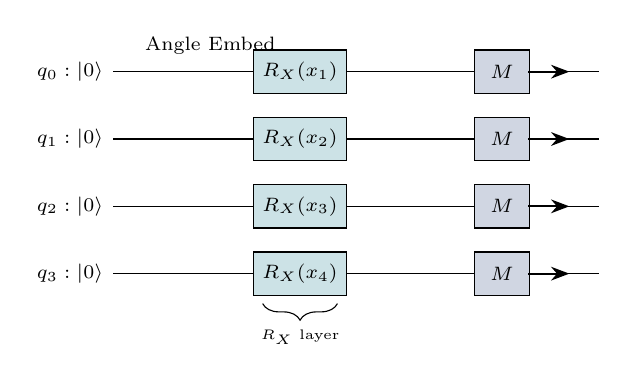
\begin{tikzpicture}[
  gate/.style={draw, fill=quantumteal!20, minimum width=0.9cm, minimum height=0.55cm, font=\scriptsize},
  meas/.style={draw, fill=auditblue!20, minimum width=0.7cm, minimum height=0.55cm, font=\scriptsize},
  scale=0.95
]
\foreach \q/\y in {0/0, 1/-0.9, 2/-1.8, 3/-2.7}{
  \draw (0, \y) -- (6.5, \y);
  \node[left, font=\scriptsize] at (0, \y) {$q_\q: |0\rangle$};
}
\foreach \q/\y/\k in {0/0/1, 1/-0.9/2, 2/-1.8/3, 3/-2.7/4}{
  \node[gate] at (2.5, \y) {$R_X(x_\k)$};
}
\foreach \q/\y in {0/0, 1/-0.9, 2/-1.8, 3/-2.7}{
  \node[meas] at (5.2, \y) {$M$};
  \draw[-Stealth, thick] (5.55, \y) -- (6.1, \y);
}
\node[font=\scriptsize] at (1.3, 0.35) {Angle Embed};
\draw[decorate, decoration={brace, mirror, amplitude=6pt}] (2.0, -3.1) -- (3.0, -3.1) node[midway, below=6pt, font=\tiny] {$R_X$ layer};
\end{tikzpicture}
\caption{Angle Embedding quantum circuit (4-qubit schematic). Each qubit $q_k$ receives an $R_X(x_k)$ rotation. The full implementation uses 8 qubits, one per PCA component. The released noise experiment replaces $R_X$ with $R_Y$ (Section~\ref{sec:noise}).}
\label{fig:circuit}
\end{figure}

% ============================================================
\section{Empirical Results and In-Depth Discussion}
\label{sec:results}
% ============================================================

\subsection{Exact Numerical Reproduction of Published Baseline}
\label{sec:repro}

Table~\ref{tab:perf42} reports full diagnostic metrics at seed=42 on WDBC and WBCO. All 36 published WDBC values (three decimals) are reproduced exactly. On WDBC, Classical RBF-SVM achieves the top accuracy ($0.9701$), followed by QSVM-Angle and OOF Stacking (both $0.9649$). RBF yields TN=201, FP=11, FN=6, TP=351 ($\text{MCC} = 0.936$; Fig.~\ref{fig:confmat}). An exact McNemar test finds no significant difference between RBF and Stacking at seed 42 (WDBC: $b=7$, $c=4$, $p=0.549$; WBCO: $b=3$, $c=3$, $p=1.0$).

\begin{table*}[!t]
\caption{Full Diagnostic Performance at Seed=42: WDBC ($N=569$, top) and WBCO ($N=683$, bottom). Positive class = benign (class 1); Specificity = malignant detection rate. Bold denotes best per column.}
\label{tab:perf42}
\centering
\footnotesize
\renewcommand{\arraystretch}{1.15}
\begin{tabularx}{\textwidth}{l *{9}{>{\centering\arraybackslash}X}}
\toprule
\multicolumn{10}{c}{\textbf{WDBC Cohort} ($N=569$, Malignant = 212, Benign = 357)} \\
\midrule
\textbf{Model Architecture} & \textbf{Accuracy} & \textbf{Precision} & \textbf{Recall} & \textbf{Specificity} & \textbf{MCC} & \textbf{TN} & \textbf{FP} & \textbf{FN} & \textbf{TP} \\
\midrule
Classical RBF-SVM & \textbf{0.9701} & \textbf{0.9696} & 0.9832 & \textbf{0.9481} & \textbf{0.9360} & \textbf{201} & \textbf{11} & 6 & 351 \\
QSVM (Angle)      & 0.9649 & 0.9542 & 0.9916 & 0.9198 & 0.9251 & 195 & 17 & 3 & 354 \\
QSVM (ZZ Map)     & 0.9596 & 0.9639 & 0.9720 & 0.9387 & 0.9134 & 199 & 13 & 10 & 347 \\
QSVM (Amplitude)  & 0.9543 & 0.9344 & \textbf{0.9972} & 0.8821 & 0.9038 & 187 & 25 & \textbf{1} & \textbf{356} \\
QKNN (Angle)      & 0.9578 & 0.9512 & 0.9832 & 0.9151 & 0.9097 & 194 & 18 & 6 & 351 \\
QKNN (ZZ Map)     & 0.9490 & 0.9362 & 0.9860 & 0.8868 & 0.8913 & 188 & 24 & 5 & 352 \\
QKNN (Amplitude)  & 0.9525 & 0.9412 & 0.9860 & 0.8962 & 0.8987 & 190 & 22 & 5 & 352 \\
Hard Voting Ens.  & 0.9613 & 0.9539 & 0.9860 & 0.9198 & 0.9173 & 195 & 17 & 5 & 352 \\
OOF Stacking Ens. & 0.9649 & 0.9668 & 0.9776 & 0.9434 & 0.9246 & 200 & 12 & 8 & 349 \\
\midrule
\multicolumn{10}{c}{\textbf{WBCO Extension Cohort} ($N=683$, Malignant = 239, Benign = 444, 16 missing dropped)} \\
\midrule
\textbf{Model Architecture} & \textbf{Accuracy} & \textbf{Precision} & \textbf{Recall} & \textbf{Specificity} & \textbf{MCC} & \textbf{TN} & \textbf{FP} & \textbf{FN} & \textbf{TP} \\
\midrule
Classical RBF-SVM & 0.9663 & 0.9817 & 0.9662 & 0.9665 & 0.9267 & 231 & 8 & 15 & 429 \\
QSVM (Angle)      & \textbf{0.9693} & 0.9818 & 0.9707 & 0.9665 & \textbf{0.9329} & 231 & 8 & 13 & 431 \\
QSVM (ZZ Map)     & 0.9649 & \textbf{0.9930} & 0.9527 & \textbf{0.9874} & 0.9256 & \textbf{236} & \textbf{3} & 21 & 423 \\
QSVM (Amplitude)  & 0.9605 & 0.9685 & 0.9707 & 0.9414 & 0.9130 & 225 & 14 & 13 & 431 \\
QKNN (Angle)      & \textbf{0.9693} & 0.9753 & 0.9775 & 0.9540 & 0.9324 & 228 & 11 & 10 & 434 \\
QKNN (ZZ Map)     & 0.9546 & 0.9519 & \textbf{0.9797} & 0.9079 & 0.8998 & 217 & 22 & \textbf{9} & \textbf{435} \\
QKNN (Amplitude)  & 0.9634 & 0.9729 & 0.9707 & 0.9498 & 0.9196 & 227 & 12 & 13 & 431 \\
Hard Voting Ens.  & 0.9663 & 0.9817 & 0.9662 & 0.9665 & 0.9267 & 231 & 8 & 15 & 429 \\
OOF Stacking Ens. & 0.9663 & 0.9795 & 0.9685 & 0.9623 & 0.9265 & 230 & 9 & 14 & 430 \\
\bottomrule
\end{tabularx}
\end{table*}

% ============================================================
% FIGURE: Confusion Matrix Heatmap
% ============================================================
\begin{figure}[!t]
\centering
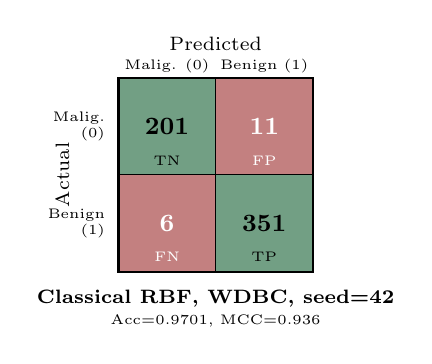
\begin{tikzpicture}[scale=0.95]
\def\cellsize{1.3}

\fill[auditgreen!60] (0,\cellsize) rectangle (\cellsize, 2*\cellsize);
\node[font=\small\bfseries] at (0.5*\cellsize, 1.5*\cellsize) {201};
\node[font=\tiny] at (0.5*\cellsize, 1.15*\cellsize) {TN};

\fill[auditred!55] (\cellsize,\cellsize) rectangle (2*\cellsize, 2*\cellsize);
\node[font=\small\bfseries, white] at (1.5*\cellsize, 1.5*\cellsize) {11};
\node[font=\tiny, white] at (1.5*\cellsize, 1.15*\cellsize) {FP};

\fill[auditred!55] (0,0) rectangle (\cellsize, \cellsize);
\node[font=\small\bfseries, white] at (0.5*\cellsize, 0.5*\cellsize) {6};
\node[font=\tiny, white] at (0.5*\cellsize, 0.16*\cellsize) {FN};

\fill[auditgreen!60] (\cellsize,0) rectangle (2*\cellsize, \cellsize);
\node[font=\small\bfseries] at (1.5*\cellsize, 0.5*\cellsize) {351};
\node[font=\tiny] at (1.5*\cellsize, 0.16*\cellsize) {TP};

\node[font=\scriptsize, rotate=90] at (-0.75, \cellsize) {Actual};
\node[font=\tiny, align=right, anchor=east] at (-0.05, 1.5*\cellsize) {Malig.\\(0)};
\node[font=\tiny, align=right, anchor=east] at (-0.05, 0.5*\cellsize) {Benign\\(1)};
\node[font=\scriptsize] at (\cellsize, 2.35*\cellsize) {Predicted};
\node[font=\tiny] at (0.5*\cellsize, 2.12*\cellsize) {Malig. (0)};
\node[font=\tiny] at (1.5*\cellsize, 2.12*\cellsize) {Benign (1)};

\draw[black, thick] (0,0) rectangle (2*\cellsize, 2*\cellsize);
\draw[black] (\cellsize, 0) -- (\cellsize, 2*\cellsize);
\draw[black] (0, \cellsize) -- (2*\cellsize, \cellsize);

\node[font=\scriptsize\bfseries] at (\cellsize, -0.35) {Classical RBF, WDBC, seed=42};
\node[font=\tiny] at (\cellsize, -0.65) {Acc=0.9701, MCC=0.936};
\end{tikzpicture}
\caption{Confusion matrix for Classical RBF-SVM on WDBC (seed=42). Rows are true classes, columns predictions; benign (class 1) is the positive class. Green: correct (TN=201 malignant, TP=351 benign). Red: errors (FP=11 malignant cases predicted benign; FN=6 benign cases predicted malignant). $\text{MCC} = 0.936$.}
\label{fig:confmat}
\end{figure}

\subsection{Multi-Seed Statistical Robustness}
\label{sec:multiseed}

Table~\ref{tab:multiseed} summarizes 10-seed accuracy distributions ($s \in \{0, 1, 2, 3, 4, 5, 10, 42, 100, 999\}$; outer and inner CV share the seed). On WDBC, Classical RBF-SVM achieves mean accuracy $0.9731 \pm 0.0017$ and outperforms OOF Stacking ($0.9670 \pm 0.0031$) in all 10 seeds (10W/0T/0L; mean gap $-0.0062$, range $-0.0123$ to $-0.0035$). On WBCO, RBF achieves $0.9690 \pm 0.0013$ vs.\ Stacking $0.9662 \pm 0.0022$, with 7 wins, 3 ties and 0 losses (Table~\ref{tab:wbco_seeds}). Across both datasets, Classical RBF equals or outperforms Stacking in \textbf{20 out of 20 seeds}. Figs.~\ref{fig:multiseed_bar} and \ref{fig:perseed} visualize these results.

\begin{table*}[!t]
\caption{Multi-Seed Accuracy Summary Across 10 Stratified 10-Fold CV Seeds ($s \in \{0, 1, 2, 3, 4, 5, 10, 42, 100, 999\}$); Std Uses $n-1$}
\label{tab:multiseed}
\centering
\footnotesize
\renewcommand{\arraystretch}{1.15}
\begin{tabularx}{\textwidth}{l *{4}{>{\centering\arraybackslash}X}}
\toprule
\textbf{Model Architecture} & \textbf{WDBC Mean $\pm$ Std} & \textbf{WDBC Range [Min, Max]} & \textbf{WBCO Mean $\pm$ Std} & \textbf{WBCO Range [Min, Max]} \\
\midrule
Classical RBF-SVM & $\mathbf{0.9731 \pm 0.0017}$ & $[0.9701, 0.9754]$ & $\mathbf{0.9690 \pm 0.0013}$ & $[0.9663, 0.9707]$ \\
QSVM (Angle)      & $0.9687 \pm 0.0023$ & $[0.9649, 0.9736]$ & $0.9685 \pm 0.0019$ & $[0.9649, 0.9707]$ \\
QSVM (ZZ Map)     & $0.9608 \pm 0.0026$ & $[0.9561, 0.9649]$ & $0.9638 \pm 0.0016$ & $[0.9605, 0.9649]$ \\
QSVM (Amplitude)  & $0.9552 \pm 0.0022$ & $[0.9525, 0.9596]$ & $0.9612 \pm 0.0012$ & $[0.9590, 0.9634]$ \\
QKNN (Angle)      & $0.9564 \pm 0.0032$ & $[0.9508, 0.9613]$ & $0.9660 \pm 0.0025$ & $[0.9619, 0.9693]$ \\
QKNN (ZZ Map)     & $0.9489 \pm 0.0027$ & $[0.9438, 0.9525]$ & $0.9511 \pm 0.0043$ & $[0.9429, 0.9561]$ \\
QKNN (Amplitude)  & $0.9480 \pm 0.0032$ & $[0.9420, 0.9525]$ & $0.9625 \pm 0.0012$ & $[0.9605, 0.9649]$ \\
Hard Voting Ens.  & $0.9638 \pm 0.0028$ & $[0.9613, 0.9701]$ & $0.9654 \pm 0.0010$ & $[0.9634, 0.9663]$ \\
OOF Stacking Ens. & $0.9670 \pm 0.0031$ & $[0.9596, 0.9701]$ & $0.9662 \pm 0.0022$ & $[0.9619, 0.9693]$ \\
\bottomrule
\end{tabularx}
\end{table*}

\begin{table}[!t]
\caption{Per-Seed Head-to-Head Comparison on WBCO: Classical RBF vs.\ OOF Stacking Ensemble ($N=683$)}
\label{tab:wbco_seeds}
\centering
\scriptsize
\setlength{\tabcolsep}{4pt}
\renewcommand{\arraystretch}{1.15}
\begin{tabular}{cccl}
\toprule
\textbf{Seed} & \textbf{Classical RBF} & \textbf{OOF Stacking} & \textbf{Outcome (disagreements)} \\
\midrule
0   & 0.9693 & 0.9634 & RBF wins, +4 correct (6) \\
1   & 0.9693 & 0.9678 & RBF wins, +1 correct (5) \\
2   & 0.9693 & 0.9678 & RBF wins, +1 correct (5) \\
3   & 0.9678 & 0.9649 & RBF wins, +2 correct (6) \\
4   & 0.9707 & 0.9663 & RBF wins, +3 correct (5) \\
5   & 0.9693 & 0.9619 & RBF wins, +5 correct (7) \\
10  & 0.9678 & 0.9678 & Tie, equal accuracy (4) \\
42  & 0.9663 & 0.9663 & Tie, equal accuracy (6) \\
100 & 0.9693 & 0.9693 & Tie, equal accuracy (2) \\
999 & 0.9707 & 0.9663 & RBF wins, +3 correct (5) \\
\midrule
\textbf{Total} & \multicolumn{3}{c}{\textbf{7 Wins / 3 Ties / 0 Losses for Classical RBF}} \\
\bottomrule
\end{tabular}

\vspace{2pt}
{\tiny Numbers in parentheses: patients on which the two models' predictions differ. No seed yields identical predictions.\par}
\end{table}

% ============================================================
% FIGURE: Multi-Seed Accuracy Bar Chart
% ============================================================
\begin{figure*}[!t]
\centering
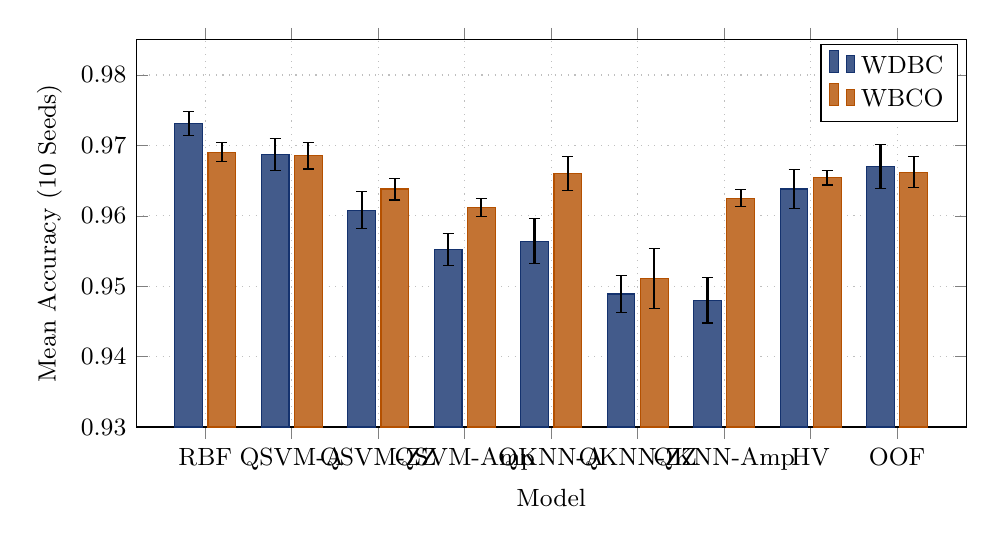
\begin{tikzpicture}
\begin{axis}[
  ybar=2pt,
  bar width=10pt,
  width=\textwidth, height=6.5cm,
  xlabel={\small Model},
  ylabel={\small Mean Accuracy (10 Seeds)},
  symbolic x coords={RBF,QSVM-A,QSVM-ZZ,QSVM-Amp,QKNN-A,QKNN-ZZ,QKNN-Amp,HV,OOF},
  xtick=data,
  xticklabel style={font=\small, rotate=0},
  ymin=0.930, ymax=0.985,
  ytick={0.930,0.940,0.950,0.960,0.970,0.980},
  yticklabel style={font=\small, /pgf/number format/fixed, /pgf/number format/precision=3},
  legend style={at={(0.99,0.99)}, anchor=north east, font=\small},
  grid=major, grid style={dotted, gray!50},
  error bars/y dir=both,
  error bars/y explicit,
  label style={font=\small}
]
\addplot+[
  fill=auditblue!80, draw=auditblue,
  error bars/error bar style={color=black, line width=0.8pt}
] coordinates {
  (RBF,      0.9731) +- (0, 0.00167)
  (QSVM-A,   0.9687) +- (0, 0.00231)
  (QSVM-ZZ,  0.9608) +- (0, 0.00263)
  (QSVM-Amp, 0.9552) +- (0, 0.00223)
  (QKNN-A,   0.9564) +- (0, 0.00319)
  (QKNN-ZZ,  0.9489) +- (0, 0.00268)
  (QKNN-Amp, 0.9480) +- (0, 0.00323)
  (HV,       0.9638) +- (0, 0.00277)
  (OOF,      0.9670) +- (0, 0.00308)
};
\addlegendentry{WDBC}

\addplot+[
  fill=classicalorange!80, draw=classicalorange,
  error bars/error bar style={color=black, line width=0.8pt}
] coordinates {
  (RBF,      0.9690) +- (0, 0.00135)
  (QSVM-A,   0.9685) +- (0, 0.00186)
  (QSVM-ZZ,  0.9638) +- (0, 0.00155)
  (QSVM-Amp, 0.9612) +- (0, 0.00124)
  (QKNN-A,   0.9660) +- (0, 0.00247)
  (QKNN-ZZ,  0.9511) +- (0, 0.00427)
  (QKNN-Amp, 0.9625) +- (0, 0.00123)
  (HV,       0.9654) +- (0, 0.00102)
  (OOF,      0.9662) +- (0, 0.00223)
};
\addlegendentry{WBCO}
\end{axis}
\end{tikzpicture}
\caption{Multi-seed (10-seed) mean accuracy with $\pm 1\sigma$ error bars for all nine models on WDBC (blue) and WBCO (orange). Classical RBF-SVM achieves the highest mean accuracy on WDBC ($0.9731$) and WBCO ($0.9690$). OOF Stacking does not surpass RBF on either dataset.}
\label{fig:multiseed_bar}
\end{figure*}

% ============================================================
% FIGURE: Per-Seed RBF vs Stacking Line Chart
% ============================================================
\begin{figure*}[!t]
\centering
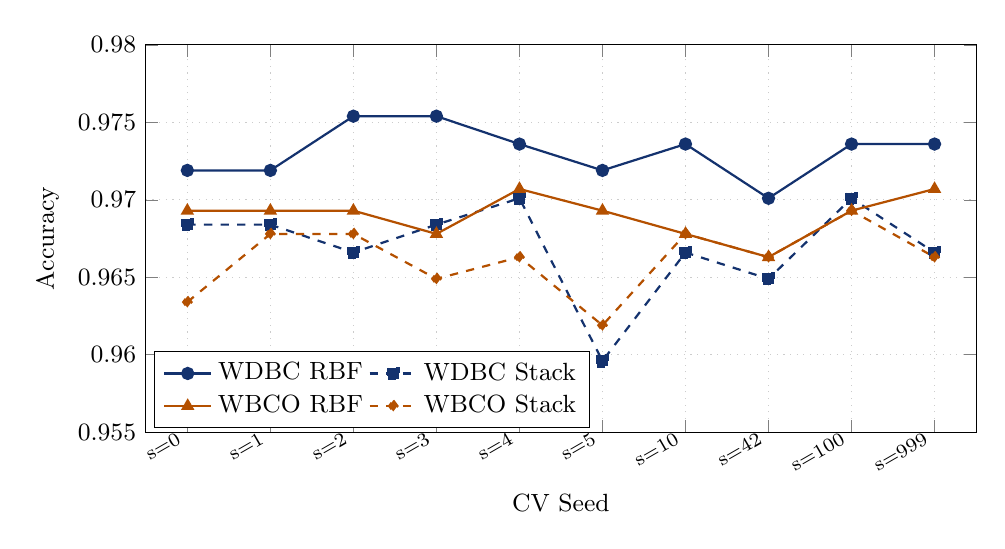
\begin{tikzpicture}
\begin{axis}[
  width=\textwidth, height=6.5cm,
  xlabel={\small CV Seed},
  ylabel={\small Accuracy},
  xmin=0.5, xmax=10.5,
  ymin=0.955, ymax=0.980,
  xtick={1,2,3,4,5,6,7,8,9,10},
  xticklabels={s=0,s=1,s=2,s=3,s=4,s=5,s=10,s=42,s=100,s=999},
  xticklabel style={font=\scriptsize, rotate=30, anchor=east},
  ytick={0.955,0.960,0.965,0.970,0.975,0.980},
  yticklabel style={font=\small, /pgf/number format/fixed, /pgf/number format/precision=3},
  grid=major, grid style={dotted, gray!40},
  legend style={at={(0.01,0.01)}, anchor=south west, font=\small, legend columns=2},
  label style={font=\small}
]
\addplot[color=auditblue, thick, mark=*, mark size=2pt]
  coordinates {(1,0.9719)(2,0.9719)(3,0.9754)(4,0.9754)(5,0.9736)(6,0.9719)(7,0.9736)(8,0.9701)(9,0.9736)(10,0.9736)};
\addlegendentry{WDBC RBF}

\addplot[color=auditblue, thick, dashed, mark=square*, mark size=2pt]
  coordinates {(1,0.9684)(2,0.9684)(3,0.9666)(4,0.9684)(5,0.9701)(6,0.9596)(7,0.9666)(8,0.9649)(9,0.9701)(10,0.9666)};
\addlegendentry{WDBC Stack}

\addplot[color=classicalorange, thick, mark=triangle*, mark size=2pt]
  coordinates {(1,0.9693)(2,0.9693)(3,0.9693)(4,0.9678)(5,0.9707)(6,0.9693)(7,0.9678)(8,0.9663)(9,0.9693)(10,0.9707)};
\addlegendentry{WBCO RBF}

\addplot[color=classicalorange, thick, dashed, mark=diamond*, mark size=2pt]
  coordinates {(1,0.9634)(2,0.9678)(3,0.9678)(4,0.9649)(5,0.9663)(6,0.9619)(7,0.9678)(8,0.9663)(9,0.9693)(10,0.9663)};
\addlegendentry{WBCO Stack}
\end{axis}
\end{tikzpicture}
\caption{Per-seed accuracy of Classical RBF (solid) vs.\ OOF Stacking (dashed) on WDBC (blue) and WBCO (orange). RBF equals or exceeds Stacking in all 20 evaluations.}
\label{fig:perseed}
\end{figure*}

\subsection{Familywise Error Control via Holm--Bonferroni Audit}
\label{sec:holm}

Table~\ref{tab:holm} and Fig.~\ref{fig:holm} summarize the 32-hypothesis bootstrap audit ($B=10{,}000$, Eq.~\eqref{eq:bootstrap_p}). On WDBC, 14 of 32 raw $p$-values fall below 0.05, and 8 survive Holm correction; all 8 show quantum models with significantly \emph{lower} precision and specificity (i.e., more malignant cases predicted benign) than RBF. On WBCO, 9 raw $p$-values fall below 0.05 and 2 survive (QKNN-ZZ precision and specificity), again both quantum-inferior. \textbf{No quantum-superior result survives on either dataset.} The stacking ensemble attains Holm $p = 1.0$ on all four metrics on both datasets (WDBC raw accuracy $p=0.449$; WBCO $p=1.0$).

\textbf{Bootstrap-seed sensitivity.} An earlier analysis with $B=1{,}000$ resamples and an uncorrected $p$-value (allowing $\hat{p}=0$) reported WBCO QKNN-Angle recall as a surviving quantum-superior result. This was an artifact of bootstrap seed 42, which happened to yield no resample with $\delta^{(b)}\le0$. At bootstrap seeds 0, 1, 7 and 123 the same test gives raw $p \in [0.012, 0.018]$, and at $B=10{,}000$ the raw $p$ is $0.013$ (Holm $p = 0.358$) for every seed tested. The underlying difference is five benign patients classified correctly by QKNN-Angle but not by RBF, and none the other way round (exact McNemar $p = 0.0625$, uncorrected).

\begin{table}[!t]
\caption{Holm--Bonferroni Survivors Among 32 Hypotheses vs.\ Classical RBF (Seed 42, $B=10{,}000$, FWER $\alpha = 0.05$)}
\label{tab:holm}
\centering
\scriptsize
\setlength{\tabcolsep}{2.5pt}
\renewcommand{\arraystretch}{1.15}
\begin{tabular}{l l l c c c l}
\toprule
\textbf{Cohort} & \textbf{Model} & \textbf{Metric} & \textbf{$\Delta$} & \textbf{Raw $p$} & \textbf{Holm $p$} & \textbf{Direction} \\
\midrule
WDBC & QSVM-Amp   & Prec. & $-0.035$ & 0.0002 & 0.0064 & Q Inferior \\
WDBC & QSVM-Amp   & Spec. & $-0.066$ & 0.0002 & 0.0064 & Q Inferior \\
WDBC & QKNN-ZZ    & Prec. & $-0.033$ & 0.0002 & 0.0064 & Q Inferior \\
WDBC & QKNN-ZZ    & Spec. & $-0.061$ & 0.0002 & 0.0064 & Q Inferior \\
WDBC & QKNN-Angle & Prec. & $-0.018$ & 0.0010 & 0.0280 & Q Inferior \\
WDBC & QKNN-Amp   & Prec. & $-0.028$ & 0.0010 & 0.0280 & Q Inferior \\
WDBC & QKNN-Amp   & Spec. & $-0.052$ & 0.0010 & 0.0280 & Q Inferior \\
WDBC & QKNN-Angle & Spec. & $-0.033$ & 0.0014 & 0.0350 & Q Inferior \\
\midrule
WBCO & QKNN-ZZ    & Prec. & $-0.030$ & 0.0002 & 0.0064 & Q Inferior \\
WBCO & QKNN-ZZ    & Spec. & $-0.059$ & 0.0002 & 0.0064 & Q Inferior \\
\bottomrule
\end{tabular}

\vspace{2pt}
{\tiny $\Delta$ = quantum minus RBF metric at seed 42. Source: \texttt{audit\_results/v3\_corrections/holm\_bootstrap\_B10000\_*.csv}.\par}
\end{table}

% ============================================================
% FIGURE: Holm p-value Scatter (WBCO, real values)
% ============================================================
\begin{figure}[!t]
\centering
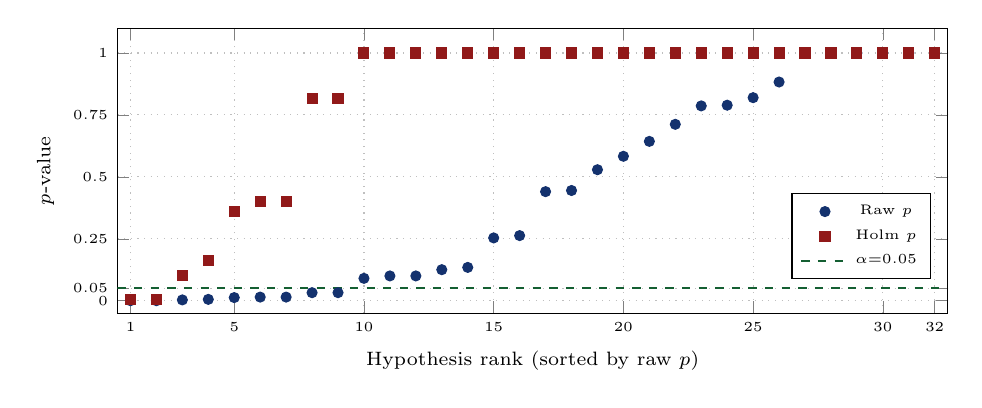
\begin{tikzpicture}
\begin{axis}[
  width=\columnwidth, height=5.2cm,
  xlabel={\scriptsize Hypothesis rank (sorted by raw $p$)},
  ylabel={\scriptsize $p$-value},
  xmin=0.5, xmax=32.5,
  ymin=-0.05, ymax=1.1,
  xtick={1,5,10,15,20,25,30,32},
  ytick={0,0.05,0.25,0.5,0.75,1.0},
  yticklabel style={/pgf/number format/fixed},
  grid=major, grid style={dotted, gray!50},
  legend style={font=\tiny, at={(0.98,0.12)}, anchor=south east},
  tick label style={font=\tiny},
  label style={font=\scriptsize}
]
\addplot[only marks, mark=*, mark size=1.8pt, color=auditblue]
  coordinates {(1,0.0002)(2,0.0002)(3,0.0034)(4,0.0056)(5,0.0128)(6,0.0148)(7,0.0148)(8,0.0326)(9,0.0326)(10,0.0904)(11,0.1002)(12,0.1002)(13,0.1254)(14,0.1346)(15,0.2536)(16,0.2630)(17,0.4404)(18,0.4450)(19,0.5289)(20,0.5831)(21,0.6433)(22,0.7121)(23,0.7865)(24,0.7893)(25,0.8197)(26,0.8829)(27,1.0000)(28,1.0000)(29,1.0000)(30,1.0000)(31,1.0000)(32,1.0000)};
\addlegendentry{Raw $p$}

\addplot[only marks, mark=square*, mark size=1.8pt, color=auditred]
  coordinates {(1,0.0064)(2,0.0064)(3,0.1020)(4,0.1624)(5,0.3584)(6,0.3996)(7,0.3996)(8,0.8149)(9,0.8149)(10,1.0000)(11,1.0000)(12,1.0000)(13,1.0000)(14,1.0000)(15,1.0000)(16,1.0000)(17,1.0000)(18,1.0000)(19,1.0000)(20,1.0000)(21,1.0000)(22,1.0000)(23,1.0000)(24,1.0000)(25,1.0000)(26,1.0000)(27,1.0000)(28,1.0000)(29,1.0000)(30,1.0000)(31,1.0000)(32,1.0000)};
\addlegendentry{Holm $p$}

\addplot[dashed, color=auditgreen, thick] coordinates {(0.5,0.05)(32.5,0.05)};
\addlegendentry{$\alpha{=}0.05$}
\end{axis}
\end{tikzpicture}
\caption{Raw (blue) and Holm-adjusted (red) bootstrap $p$-values for the 32 WBCO hypotheses ($B=10{,}000$). Nine raw $p$-values lie below $\alpha=0.05$ (dashed); only two (QKNN-ZZ precision and specificity, both quantum-inferior) remain below it after Holm correction.}
\label{fig:holm}
\end{figure}

\subsection{Fold-Local Preprocessing Audit (TOST)}
\label{sec:tost}

The TOST audit compares the released global preprocessing with strictly fold-local fitting for the OOF Stacking ensemble:
\begin{itemize}
    \item \textbf{WDBC}: Global accuracy $0.96485$ (549/569), fold-local $0.96661$ (550/569), $\Delta = +0.00176$. Concordance $98.77\%$ (562/569). McNemar $b=3$, $c=4$, $p = 1.0$. TOST $p = 0.0385$; 90\% CI of $\Delta$: $[-0.0059, 0.0094]$, inside $\pm0.01$.
    \item \textbf{WBCO}: Global accuracy $0.96633$ (660/683), fold-local $0.96779$ (661/683), $\Delta = +0.00146$. Concordance $99.56\%$ (680/683). McNemar $b=1$, $c=2$, $p = 1.0$. TOST $p = 0.0004$.
\end{itemize}
Fold-local fitting does not lower accuracy on either dataset, so global preprocessing did not inflate the published results. The WDBC equivalence is narrow: the 95\% paired-bootstrap interval $[-0.0070, 0.0105]$ slightly exceeds the margin.

\subsection{Classical Baseline Fairness}
\label{sec:fairness}

Table~\ref{tab:fairness} reports classical baselines on WDBC at seed 42, released (default) and tuned by nested grid search (inner stratified 5-fold \texttt{GridSearchCV}; for RBF, $C \in \{0.1, 1, 10, 100\}$, $\gamma \in \{\text{scale}, \text{auto}, 0.01, 0.1, 1\}$). Tuning raises RBF accuracy from $0.9701$ to $0.9719$. Neither tuned nor untuned RBF differs significantly from the quantum stacking ensemble (McNemar $p = 0.424$ and $p=0.549$), but both are numerically ahead. The untuned baseline therefore did not disadvantage the quantum ensemble in this benchmark; it understated the classical ceiling only slightly.

\begin{table}[!t]
\caption{Classical Baselines on WDBC (Seed 42) vs.\ Quantum OOF Stacking (Accuracy $0.9649$)}
\label{tab:fairness}
\centering
\scriptsize
\setlength{\tabcolsep}{3pt}
\renewcommand{\arraystretch}{1.12}
\begin{tabular}{lccc}
\toprule
\textbf{Model} & \textbf{Acc.} & \textbf{$\Delta$ vs.\ Q-Stack} & \textbf{McNemar $p$} \\
\midrule
RBF-SVM (released)          & 0.9701 & $+0.0053$ & 0.549 \\
RBF-SVM (tuned)             & \textbf{0.9719} & $+0.0070$ & 0.424 \\
XGBoost (released)          & 0.9684 & $+0.0035$ & 0.832 \\
XGBoost (tuned)             & 0.9649 & $\phantom{+}0.0000$ & 1.000 \\
Random Forest (released)    & 0.9473 & $-0.0176$ & 0.064 \\
Random Forest (tuned)       & 0.9455 & $-0.0193$ & 0.035 \\
Classical Stack (released) & 0.9666 & $+0.0018$ & 1.000 \\
Classical Stack (tuned)  & 0.9684 & $+0.0035$ & 0.688 \\
\bottomrule
\end{tabular}

\vspace{2pt}
{\tiny Source: \texttt{audit\_results/classical\_fairness/}. Raw McNemar $p$, uncorrected.\par}
\end{table}

\subsection{Algorithmic Model Selection Audit}
\label{sec:selection}

We replace the fixed quartet with nested selection: within each outer fold, all $\binom{6}{4}=15$ four-model subsets are scored on inner OOF predictions by three criteria (validation accuracy, balanced accuracy and meta-learner CV accuracy), and the best subset is stacked. Table~\ref{tab:selection} reports how often QSVM-Angle and the published quartet are chosen; Fig.~\ref{fig:selection_heatmap} shows the WBCO selections under the accuracy criterion.

\begin{table}[!t]
\caption{Nested Selection Frequency over 10 Outer Folds: Folds Including QSVM-Angle / Folds Selecting the Published Quartet}
\label{tab:selection}
\centering
\scriptsize
\setlength{\tabcolsep}{4pt}
\renewcommand{\arraystretch}{1.15}
\begin{tabular}{lcccc}
\toprule
& \multicolumn{2}{c}{\textbf{WDBC}} & \multicolumn{2}{c}{\textbf{WBCO}} \\
\cmidrule(lr){2-3}\cmidrule(lr){4-5}
\textbf{Criterion} & \textbf{QSVM-Angle} & \textbf{Quartet} & \textbf{QSVM-Angle} & \textbf{Quartet} \\
\midrule
Validation accuracy & 10/10 & 0/10 & 10/10 & 0/10 \\
Balanced accuracy   & 10/10 & 0/10 & 10/10 & 0/10 \\
Meta-CV accuracy    & 8/10  & 1/10 & 9/10  & 1/10 \\
\bottomrule
\end{tabular}
\end{table}

QSVM-Angle is the single most accurate quantum base model in every WDBC outer fold (inner validation accuracy $0.9610$--$0.9746$). The published quartet is selected only once per dataset, and on WDBC that selection is an exact score tie (gap $0.0000$) with identical outer-test predictions. However, the selection is unstable---the modal subset recurs in only 30--60\% of WDBC folds, with winning margins of 1--2 training samples---and its effect on accuracy is not significant: on WDBC, accuracy-selected stacking reaches $0.9684$ vs.\ $0.9649$ for the fixed quartet (paired bootstrap $p=0.578$; McNemar $p=0.727$), and meta-CV selection reaches $0.9613$ ($p=0.572$; McNemar $p=0.688$).

\begin{remark}
The authors state that the quartet was chosen to maximize diversity over encoding geometry and classifier type, a constrained objective that an unconstrained accuracy search does not enforce. The audit therefore shows that the quartet is a fixed, a priori design choice rather than an adaptive, data-driven selection, and that it omits the strongest base model; it does not show that the choice degrades accuracy.
\end{remark}

% ============================================================
% FIGURE: Model Selection Inclusion Heatmap (WBCO, accuracy criterion)
% ============================================================
\begin{figure}[!t]
\centering
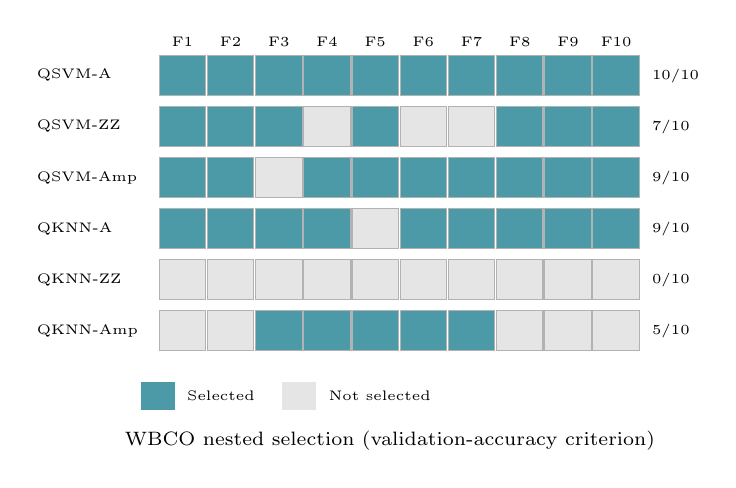
\begin{tikzpicture}[scale=0.72, every node/.style={font=\tiny}]
\foreach \f in {1,...,10}{
  \node at (\f*0.85 - 0.11, 4.5) {F\f};
}
% rows: name / y / per-fold inclusion (F1..F10) / count
\foreach \name/\y/\pattern/\cnt in {
  QSVM-A/3.55/{1,1,1,1,1,1,1,1,1,1}/10,
  QSVM-ZZ/2.65/{1,1,1,0,1,0,0,1,1,1}/7,
  QSVM-Amp/1.75/{1,1,0,1,1,1,1,1,1,1}/9,
  QKNN-A/0.85/{1,1,1,1,0,1,1,1,1,1}/9,
  QKNN-ZZ/-0.05/{0,0,0,0,0,0,0,0,0,0}/0,
  QKNN-Amp/-0.95/{0,0,1,1,1,1,1,0,0,0}/5}{
  \node[right, font=\tiny] at (-2.0, \y+0.35) {\name};
  \node[right, font=\tiny] at (8.85, \y+0.35) {\cnt/10};
  \foreach \v [count=\f] in \pattern {
    \ifnum\v=1
      \fill[quantumteal!70] (\f*0.85 - 0.52, \y) rectangle (\f*0.85 + 0.30, \y+0.7);
    \else
      \fill[gray!20] (\f*0.85 - 0.52, \y) rectangle (\f*0.85 + 0.30, \y+0.7);
    \fi
    \draw[gray!60] (\f*0.85 - 0.52, \y) rectangle (\f*0.85 + 0.30, \y+0.7);
  }
}
\fill[quantumteal!70] (0.0, -2.0) rectangle (0.6, -1.5);
\node[right] at (0.65, -1.75) {Selected};
\fill[gray!20] (2.5, -2.0) rectangle (3.1, -1.5);
\node[right] at (3.15, -1.75) {Not selected};
\node[below, font=\scriptsize] at (4.4, -2.2) {WBCO nested selection (validation-accuracy criterion)};
\end{tikzpicture}
\caption{Base models in the selected 4-model subset per outer fold on WBCO (validation-accuracy criterion). QSVM-Angle is selected in all 10 folds; the published quartet (QSVM-Amp, QKNN-Amp, QSVM-ZZ, QKNN-Angle) is never the selected subset under this criterion. Source: \texttt{audit\_results/wbco/wbco\_model\_selection\_nested\_audit.csv}.}
\label{fig:selection_heatmap}
\end{figure}

\subsection{Noise Simulation Audit}
\label{sec:noise}

\textbf{Circuit mismatch.} The released noise experiment uses PennyLane's \texttt{default.mixed} density-matrix simulator with exact Kraus channels; the trace is preserved ($\text{Tr}\,\rho = 1.000000$ in our re-execution). However, the noisy circuits are not the benchmarked feature maps. The Angle map uses $R_Y$ instead of $R_X$, and the ZZ map couples only the 7 nearest-neighbour pairs instead of all 28 pairs (14 instead of 56 two-qubit gates over the forward and adjoint circuits). Because two-qubit gates dominate hardware error, the reduced circuit understates the noise exposure of the benchmarked ZZ kernel.

\textbf{Kernel diagnostics.} Table~\ref{tab:noise} reports Gram-matrix diagonals (self-fidelities) on the 60-patient subsample. For ZZ at $p=0.05$, the released chain retains $K_{ii}\in[0.192, 0.229]$, whereas the corrected all-to-all circuit retains only $K_{ii}\in[0.0096, 0.0159]$---about $18\times$ lower on average ($0.205$ vs.\ $0.0116$)---and $[0.0042, 0.0051]$ at $p=0.10$, close to the maximally mixed value $2^{-8}=0.0039$. The noisy Amplitude Gram matrices are not positive semi-definite ($\lambda_{\min}=-0.0029$ and $-0.0058$).

\textbf{Downstream behaviour.} At both $p=0.05$ and $p=0.10$, noisy QSVM-ZZ predicts the benign class for all 60 patients (accuracy $0.633$ = majority rate, specificity $0.0$), under both the released and the corrected circuits. OOF Stacking keeps accuracy $0.933$ because the meta-learner drives the QSVM-ZZ coefficient from $0.77$--$2.17$ (clean) to $|\beta|<0.001$ in every noisy fold. The reported ensemble ``robustness'' therefore reflects the meta-learner discarding a collapsed base model, measured on circuits other than those benchmarked, on 60 patients without shot noise.

\begin{table}[!t]
\caption{Noise Audit on the Released 60-Patient WDBC Subsample (5-Fold CV)}
\label{tab:noise}
\centering
\scriptsize
\setlength{\tabcolsep}{2pt}
\renewcommand{\arraystretch}{1.12}
\begin{tabular}{lccc}
\toprule
\multicolumn{4}{l}{\textbf{(a) Gram diagonal $K_{ii}$ range (clean $K_{ii}=1$)}} \\
\midrule
\textbf{Kernel / circuit} & $p=0.05$ & $p=0.10$ & \textbf{PSD} \\
\midrule
ZZ, released 7-edge chain   & [0.192, 0.229] & [0.048, 0.067] & Yes \\
ZZ, corrected all-to-all    & [0.0096, 0.0159] & [0.0042, 0.0051] & Yes \\
Angle ($R_X$ or $R_Y$)      & 0.587 & 0.345 & Yes \\
Amplitude                   & [0.802, 0.818] & [0.644, 0.670] & No \\
\midrule
\multicolumn{4}{l}{\textbf{(b) Accuracy / Specificity (identical for both circuits)}} \\
\midrule
\textbf{Model} & $p=0$ & $p=0.05$ & $p=0.10$ \\
\midrule
QSVM (ZZ)        & 0.917 / 0.81 & 0.633 / 0.00 & 0.633 / 0.00 \\
QSVM (Angle)     & 0.933 / 0.81 & 0.950 / 0.86 & 0.900 / 0.73 \\
QKNN (Amplitude) & 0.900 / 0.73 & 0.917 / 0.78 & 0.917 / 0.78 \\
Hard Voting      & 0.917 / 0.77 & 0.917 / 0.78 & 0.900 / 0.73 \\
OOF Stacking     & 0.933 / 0.86 & 0.933 / 0.83 & 0.933 / 0.83 \\
\bottomrule
\end{tabular}

\vspace{2pt}
{\tiny Source: \texttt{audit\_results/noise\_nisq/}. Specificity = malignant detection rate.\par}
\end{table}

\subsection{Variational Classifier Gradient Audit}
\label{sec:vqc}

The audited study attributes the failure of its 8-qubit variational quantum classifier (VQC; 48 parameters) to a barren plateau. In the released cost function, circuit outputs are collected in a Python list before subtraction from the labels, which detaches them from PennyLane's autodiff graph. At the same parameters and batch, the released loss returns a gradient of exactly zero (L2 norm $0.0$; 0 of 48 components non-zero), whereas finite differences show a non-zero true gradient (maximum component $0.092$). Stacking the outputs with \texttt{pnp.stack} restores the gradient (L2 norm $0.102$; all 48 components non-zero; agreement with finite differences to $1.1\times10^{-11}$). The reported training failure is therefore a software defect, not evidence of a barren plateau.

\subsection{Probabilistic Calibration Analysis}
\label{sec:calibration}

Fig.~\ref{fig:calibration} shows reliability curves on WDBC (seed 42, 10 equal-width bins). Classical RBF-SVM (LIBSVM Platt probabilities) achieves Expected Calibration Error (ECE) $= 0.0173$ and Brier score $= 0.0233$; raw OOF Stacking is worse on both (ECE $= 0.0332$, Brier $= 0.0299$). Additional Platt scaling (\texttt{CalibratedClassifierCV}, inner 5-fold) improves Stacking to ECE $= 0.0267$ (Brier $0.0290$) but worsens RBF to ECE $= 0.0419$ (Brier $0.0260$). Calibration rankings are therefore metric-dependent, and RBF has the lower Brier score in both settings.

% ============================================================
% FIGURE: Calibration / Reliability Diagram (real bins)
% ============================================================
\begin{figure}[!t]
\centering
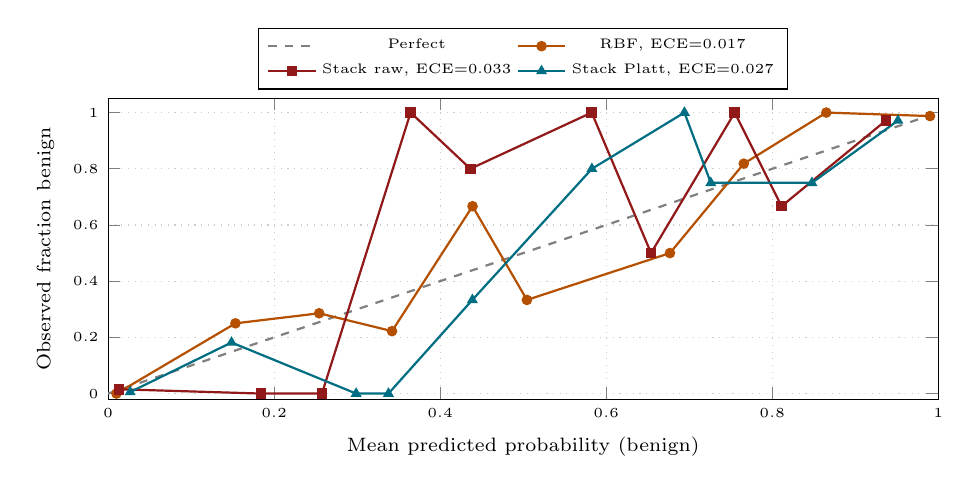
\begin{tikzpicture}
\begin{axis}[
  width=\columnwidth, height=5.4cm,
  xlabel={\scriptsize Mean predicted probability (benign)},
  ylabel={\scriptsize Observed fraction benign},
  xmin=0, xmax=1, ymin=-0.02, ymax=1.05,
  xtick={0,0.2,0.4,0.6,0.8,1.0},
  ytick={0,0.2,0.4,0.6,0.8,1.0},
  grid=major, grid style={dotted, gray!40},
  legend style={font=\tiny, at={(0.5,1.03)}, anchor=south, legend columns=2},
  tick label style={font=\tiny},
  label style={font=\scriptsize}
]
\addplot[dashed, gray, thick] coordinates {(0,0)(1,1)};
\addlegendentry{Perfect}

\addplot[color=classicalorange, thick, mark=*, mark size=1.5pt]
  coordinates {(0.0101,0.0000)(0.1534,0.2500)(0.2543,0.2857)(0.3420,0.2222)(0.4390,0.6667)(0.5045,0.3333)(0.6768,0.5000)(0.7657,0.8182)(0.8651,1.0000)(0.9900,0.9876)};
\addlegendentry{RBF, ECE=0.017}

\addplot[color=auditred, thick, mark=square*, mark size=1.5pt]
  coordinates {(0.0134,0.0154)(0.1844,0.0000)(0.2576,0.0000)(0.3644,1.0000)(0.4364,0.8000)(0.5825,1.0000)(0.6540,0.5000)(0.7548,1.0000)(0.8112,0.6667)(0.9368,0.9716)};
\addlegendentry{Stack raw, ECE=0.033}

\addplot[color=quantumteal, thick, mark=triangle*, mark size=1.5pt]
  coordinates {(0.0266,0.0054)(0.1487,0.1818)(0.2988,0.0000)(0.3377,0.0000)(0.4388,0.3333)(0.5828,0.8000)(0.6942,1.0000)(0.7260,0.7500)(0.8478,0.7500)(0.9514,0.9716)};
\addlegendentry{Stack Platt, ECE=0.027}
\end{axis}
\end{tikzpicture}
\caption{Reliability diagram on WDBC (seed 42, 10 bins; points at bin mean confidence). Most patients fall in the extreme bins (e.g., 183 and 323 of 569 for RBF); intermediate bins contain 1--17 patients, so their points are noisy. Source: \texttt{audit\_results/calibration/calibration\_reliability\_data.csv}.}
\label{fig:calibration}
\end{figure}

\subsection{Cross-Dataset Benchmark}
\label{sec:cross}

Table~\ref{tab:crossbench} compares the 10-seed results across WDBC and WBCO. Classical RBF-SVM has the top mean accuracy on both cohorts ($0.9731$ and $0.9690$), and Stacking does not surpass RBF on either.

\begin{table*}[!t]
\caption{Cross-Dataset Performance Benchmark: WDBC ($N=569$) vs.\ WBCO ($N=683$), 10-Seed Mean Accuracy}
\label{tab:crossbench}
\centering
\footnotesize
\renewcommand{\arraystretch}{1.15}
\begin{tabularx}{\textwidth}{l *{4}{>{\centering\arraybackslash}X}}
\toprule
\textbf{Model Architecture} & \textbf{WDBC 10-Seed Mean $\pm$ Std} & \textbf{WBCO 10-Seed Mean $\pm$ Std} & \textbf{Cross-Dataset $\Delta$ (WDBC $-$ WBCO)} & \textbf{Role} \\
\midrule
Classical RBF-SVM & $\mathbf{0.9731 \pm 0.0017}$ & $\mathbf{0.9690 \pm 0.0013}$ & $+0.0041$ & Classical baseline \\
QSVM (Angle)      & $0.9687 \pm 0.0023$ & $0.9685 \pm 0.0019$ & $+0.0002$ & Top individual quantum \\
QSVM (ZZ Map)     & $0.9608 \pm 0.0026$ & $0.9638 \pm 0.0016$ & $-0.0030$ & Quantum base model \\
QSVM (Amplitude)  & $0.9552 \pm 0.0022$ & $0.9612 \pm 0.0012$ & $-0.0060$ & Quantum base model \\
QKNN (Angle)      & $0.9564 \pm 0.0032$ & $0.9660 \pm 0.0025$ & $-0.0096$ & Quantum base model \\
QKNN (ZZ Map)     & $0.9489 \pm 0.0027$ & $0.9511 \pm 0.0043$ & $-0.0022$ & Quantum base model \\
QKNN (Amplitude)  & $0.9480 \pm 0.0032$ & $0.9625 \pm 0.0012$ & $-0.0145$ & Quantum base model \\
Hard Voting Ens.  & $0.9638 \pm 0.0028$ & $0.9654 \pm 0.0010$ & $-0.0016$ & 3-model vote \\
OOF Stacking Ens. & $0.9670 \pm 0.0031$ & $0.9662 \pm 0.0022$ & $+0.0008$ & \textbf{RBF wins/ties 20/20 seeds} \\
\bottomrule
\end{tabularx}
\end{table*}

\subsection{Methodological Generalization Assessment}
\label{sec:generalization}

Table~\ref{tab:generalization} summarizes generalization verdicts for the four core findings. Three are fully confirmed on WBCO (FWER audit, fold-local TOST equivalence and the selection discrepancy), and one is partially confirmed (seed robustness weakens from 10 wins to 7 wins and 3 ties, still with zero losses).

\begin{table*}[!t]
\caption{Methodological Generalization Assessment: Core Audit Findings Across Both Datasets}
\label{tab:generalization}
\centering
\footnotesize
\renewcommand{\arraystretch}{1.25}
\begin{tabularx}{\textwidth}{>{\centering\arraybackslash\bfseries}p{0.5cm} >{\raggedright\arraybackslash\bfseries}p{3.2cm} >{\raggedright\arraybackslash}p{3.8cm} >{\raggedright\arraybackslash}X >{\centering\arraybackslash\bfseries}p{2.3cm}}
\toprule
\# & Methodological Dimension & WDBC Finding ($N=569$) & WBCO Replication ($N=683$) & Generalization Verdict \\
\midrule
1 & Multi-Seed Robustness & Classical RBF wins 10 of 10 seeds (0 ties, 0 losses). Mean gap: $-0.0062$. & Classical RBF wins 7 of 10 seeds, ties 3, 0 losses. Mean gap: $-0.0028$. & \textbf{Partially Confirmed} \\
\midrule
2 & FWER Hypothesis Testing (32 Tests, Holm $\alpha = 0.05$, $B=10{,}000$) & 8 of 32 survive, all quantum-inferior (precision/specificity). Zero quantum superiority; stacking Holm $p=1.0$. & 2 of 32 survive (QKNN-ZZ precision/specificity), both quantum-inferior. Zero quantum superiority; stacking Holm $p=1.0$. & \textbf{Confirmed} \\
\midrule
3 & Fold-Local Preprocessing (TOST $\pm 1\%$) & $\Delta=+0.00176$ (+1 patient); concordance $98.77\%$; TOST $p = 0.0385$. & $\Delta=+0.00146$ (+1 patient); concordance $99.56\%$; TOST $p = 0.0004$. & \textbf{Confirmed} \\
\midrule
4 & Nested Model Selection & QSVM-Angle in 10/10 (accuracy, balanced) and 8/10 (meta-CV) folds; quartet 0/10, 0/10, 1/10. & QSVM-Angle in 10/10, 10/10, 9/10 folds; quartet 0/10, 0/10, 1/10. & \textbf{Confirmed} \\
\bottomrule
\end{tabularx}
\end{table*}

\section{Threats to Validity}
\label{sec:threats}
% ============================================================

\textbf{Internal Validity.} The audit executes the released pipeline with PennyLane 0.44.1 \cite{bergholm2018pennylane} and Scikit-Learn 1.5.2 \cite{pedregosa2011sklearn}; other versions may differ numerically. Exact reproduction of all 36 published WDBC values and of the stored WBCO OOF predictions confirms operational fidelity. Bootstrap $p$-values depend on the resampling seed; we use $B=10{,}000$ and report seed sensitivity for the one borderline result (Section~\ref{sec:holm}).

\textbf{Construct Validity.} Under the code's label convention, ``recall'' measures benign sensitivity and ``specificity'' measures malignant detection; clinically, the surviving quantum-inferior specificity results correspond to more missed malignancies. Clinical utility also depends on calibration and decision-curve analysis, which we address only partially.

\textbf{External Validity.} WDBC and WBCO are curated cytology benchmarks from the same clinical domain; results may not transfer to other oncology tasks, imaging data, or the Parkinson's and Diabetes benchmarks of the audited study. All circuits are simulated; the noise audit uses 60 patients, exact density matrices without shot noise, and a phenomenological depolarizing model, not hardware.

\textbf{Statistical Validity.} Stratified CV approximately preserves exchangeability, but OOF predictions from overlapping training sets are not independent, so bootstrap and McNemar $p$-values are approximate. Holm control is conservative by design. The TOST margin ($\pm1\%$) is audit-defined rather than clinically derived.

% ============================================================
\section{Conclusion}
\label{sec:conclusion}
% ============================================================

This paper presented an independent, code-level statistical audit of an adaptive quantum kernel stacking framework on two breast cancer cytology benchmarks. Our findings are:
\begin{enumerate}
    \item Classical RBF-SVM equals or outperforms the quantum stacking ensemble in 20 of 20 seed evaluations across WDBC and WBCO, with zero losses.
    \item Under FWER control (32 hypotheses, $B=10{,}000$), no quantum-superior result survives on either dataset; all survivors show quantum models detecting fewer malignancies than RBF, and the ensemble has Holm $p=1.0$.
    \item Preprocessing leakage is ruled out by TOST equivalence on both datasets ($p < 0.05$).
    \item The ``adaptive'' ensemble is a fixed quartet; unconstrained nested selection includes the excluded QSVM-Angle in 8--10 of 10 folds, although the resulting accuracy differences are not significant.
    \item The noise-robustness experiment simulates different circuits from those benchmarked (75\% fewer entangling gates), and its ensemble stability reflects the meta-learner discarding a collapsed QSVM-ZZ.
    \item The reported VQC barren plateau is a severed autodiff graph that yields exactly zero gradients.
\end{enumerate}

The claimed quantum advantage is not supported by rigorous statistical evidence on these benchmarks. Biomedical QML studies should report multi-seed evaluation, FWER-controlled testing, tuned classical baselines, gradient checks, and noise simulations of the benchmarked circuits.

\section*{Data and Code Availability}
WDBC is available from Scikit-Learn and the UCI repository; WBCO from the UCI repository. All audit scripts, cached Gram matrices and result tables are in the audit repository (\texttt{audit\_results/}); v3 corrections are generated by \texttt{audit\_results/scripts/run\_v3\_corrections.py}.

% ============================================================
% BIBLIOGRAPHY
% ============================================================
\begin{thebibliography}{99}

\bibitem{globocan2020}
H.~Sung, J.~Ferlay, R.~L.~Siegel, M.~Laversanne, I.~Soerjomataram, A.~Jemal, and F.~Bray,
``Global cancer statistics 2020: GLOBOCAN estimates of incidence and mortality worldwide for 36 cancers in 185 countries,''
\emph{CA: A Cancer Journal for Clinicians}, vol.~71, no.~3, pp.~209--249, 2021.

\bibitem{mangasarian1995breast}
O.~L.~Mangasarian, W.~N.~Street, and W.~H.~Wolberg,
``Breast cancer diagnosis and prognosis via linear programming,''
\emph{Operations Research}, vol.~43, no.~4, pp.~570--577, 1995.

\bibitem{street1993nuclear}
W.~N.~Street, W.~H.~Wolberg, and O.~L.~Mangasarian,
``Nuclear feature extraction for breast tumor diagnosis,''
in \emph{Proc. SPIE 1905, Biomedical Image Processing and Biomedical Visualization}, pp.~861--870, 1993.

\bibitem{wolberg1990multisurface}
W.~H.~Wolberg and O.~L.~Mangasarian,
``Multisurface method of pattern separation for medical diagnosis applied to breast cytology,''
\emph{Proceedings of the National Academy of Sciences}, vol.~87, no.~23, pp.~9193--9196, 1990.

\bibitem{preskill2018quantum}
J.~Preskill,
``Quantum computing in the NISQ era and beyond,''
\emph{Quantum}, vol.~2, p.~79, 2018.

\bibitem{biamonte2017quantum}
J.~Biamonte, P.~Wittek, N.~Pancotti, P.~Rebentrost, N.~Wiebe, and S.~Lloyd,
``Quantum machine learning,''
\emph{Nature}, vol.~549, no.~7671, pp.~195--202, 2017.

\bibitem{havlicek2019supervised}
V.~Havl{\'i}{\v c}ek, A.~D.~C{\'o}rcoles, K.~Temme, A.~W.~Harrow, A.~Kandala, J.~M.~Chow, and J.~M.~Gambetta,
``Supervised learning with quantum-enhanced feature spaces,''
\emph{Nature}, vol.~567, no.~7747, pp.~209--212, 2019.

\bibitem{schuld2019quantum}
M.~Schuld and N.~Killoran,
``Quantum machine learning in feature Hilbert spaces,''
\emph{Physical Review Letters}, vol.~122, no.~4, p.~040504, 2019.

\bibitem{liu2021rigorous}
Y.~Liu, S.~Arunachalam, and K.~Temme,
``A rigorous and robust quantum speed-up in supervised machine learning,''
\emph{Nature Physics}, vol.~17, no.~9, pp.~1013--1017, 2021.

% TODO: add author initials from the published article (not verifiable from the repository).
\bibitem{daga2026adaptive}
Daga, Naole, Parikh, Bommineni, and Ramu,
``Adaptive quantum kernel selection via leakage-free stacking for clinical diagnostics on NISQ hardware,''
\emph{Scientific Reports}, vol.~16, p.~26840, 2026.

\bibitem{rebentrost2014quantum}
P.~Rebentrost, M.~Mohseni, and S.~Lloyd,
``Quantum support vector machine for big data classification,''
\emph{Physical Review Letters}, vol.~113, no.~13, p.~130503, 2014.

\bibitem{li2015experimental}
Z.~Li, X.~Liu, N.~Xu, and J.~Du,
``Experimental realization of a quantum support vector machine,''
\emph{Physical Review Letters}, vol.~114, no.~14, p.~140504, 2015.

\bibitem{altares2021automatic}
S.~Altares-L{\'o}pez, A.~Ribeiro, and J.~J.~Garc{\'i}a-Ripoll,
``Automatic design of quantum feature maps,''
\emph{Quantum Science and Technology}, vol.~6, no.~4, p.~045015, 2021.

\bibitem{demsar2006statistical}
J.~Dem{\v s}ar,
``Statistical comparisons of classifiers over multiple data sets,''
\emph{Journal of Machine Learning Research}, vol.~7, pp.~1--30, 2006.

\bibitem{holm1979simple}
S.~Holm,
``A simple sequentially rejective multiple test procedure,''
\emph{Scandinavian Journal of Statistics}, vol.~6, no.~2, pp.~65--70, 1979.

\bibitem{efron1994introduction}
B.~Efron and R.~J.~Tibshirani,
\emph{An Introduction to the Bootstrap}.
New York: Chapman \& Hall/CRC, 1994.

\bibitem{wellek2010testing}
S.~Wellek,
\emph{Testing Statistical Hypotheses of Equivalence and Noninferiority}, 2nd~ed.
Boca Raton: CRC Press, 2010.

\bibitem{mcnemar1947note}
Q.~McNemar,
``Note on the sampling error of the difference between correlated proportions or percentages,''
\emph{Psychometrika}, vol.~12, no.~2, pp.~153--157, 1947.

\bibitem{nielsen2010quantum}
M.~A.~Nielsen and I.~L.~Chuang,
\emph{Quantum Computation and Quantum Information}.
Cambridge: Cambridge University Press, 2010.

\bibitem{cerezo2021variational}
M.~Cerezo, A.~Arrasmith, R.~Babbush, S.~C.~Benjamin, S.~Endo, K.~Fujii, J.~R.~McClean, K.~Mitarai, X.~Yuan, L.~Cincio, and P.~J.~Coles,
``Variational quantum algorithms,''
\emph{Nature Reviews Physics}, vol.~3, no.~9, pp.~625--644, 2021.

\bibitem{wolpert1992stacked}
D.~H.~Wolpert,
``Stacked generalization,''
\emph{Neural Networks}, vol.~5, no.~2, pp.~241--259, 1992.

\bibitem{bergholm2018pennylane}
V.~Bergholm, J.~Izaac, M.~Schuld, C.~Gogolin, S.~Ahmed, V.~Ajith, M.~S.~Alam, G.~Alonso-Linaje, B.~AkashNarayanan, A.~Asadi, et~al.,
``PennyLane: Automatic differentiation of hybrid quantum-classical computations,''
\emph{arXiv preprint arXiv:1811.04968}, 2018.

\bibitem{pedregosa2011sklearn}
F.~Pedregosa, G.~Varoquaux, A.~Gramfort, V.~Michel, B.~Thirion, O.~Grisel, M.~Blondel, P.~Prettenhofer, R.~Weiss, V.~Dubourg, et~al.,
``Scikit-learn: Machine learning in Python,''
\emph{Journal of Machine Learning Research}, vol.~12, pp.~2825--2830, 2011.

\bibitem{tang2019quantum}
E.~Tang,
``A quantum-inspired classical algorithm for recommendation systems,''
in \emph{Proceedings of the 51st Annual ACM STOC}, pp.~217--228, 2019.

\end{thebibliography}

\end{document}
